\documentclass[10pt]{report}
\usepackage{fancyhdr, amsmath, amsthm, amssymb, tikz, setspace}
\usepackage[font=scriptsize]{subcaption}
\usepackage[margin=0.5in, top=0.8in,bottom=0.8in]{geometry}
\usepackage[version=3]{mhchem}
\newcommand{\scinot}[2]{#1\times 10^{#2}}
\newcommand{\bra}[1]{\left<#1\right|}
\newcommand{\ket}[1]{\left|#1\right>}
\newcommand{\dotp}[2]{\left<#1\left.\right|#2\right>}
\newcommand{\rd}[2]{\frac{d#1}{d#2}}
\newcommand{\pd}[2]{\frac{\partial #1}{\partial#2}}
\newcommand{\norm}[1]{\left|\left|#1\right|\right|}
\newcommand{\ptd}[2]{\frac{\partial^2 #1}{\partial#2^2}}
\newcommand{\rtd}[2]{\frac{d^2#1}{d#2^2}}
\newcommand{\tensor}[1]{\overleftrightarrow{#1}}
\newcommand{\curl}[0]{\vec{\nabla}\times}
\newcommand{\pvec}[1]{\vec{#1}^{\,\prime}}
\newcommand{\grad}[0]{\vec{\nabla}}
\renewcommand{\div}[0]{\vec{\nabla}\cdot}
\newcommand{\expvalue}[1]{\left<#1\right>}
\newcommand{\abs}[1]{\left|#1\right|}
\usepackage[labelfont=bf, font=scriptsize]{caption}
\everymath{\displaystyle}

\begin{document}

%\doublespace
\pagestyle{fancy}
\rhead{Yubo Su - Ph106}
%\setlength{\headheight}{15pt}

\title{Ph106b - Michael Cross/Sunil Golwala - DWN107 TTh 1030-12}
\author{Yubo Su}
\date{ }

\maketitle

\tableofcontents

\chapter{Key Concepts}

Relativity; note $c=1$

\begin{itemize}
    \item Relativity is just that all laws of physics are the same in all inertial frames. We notate $c=1$.
    \item Lorentz Transform. Note that primed coordinates are moving coordinates.
        \begin{align*}
            x' &= \gamma(x-vt) & x &= \gamma(x' + vt')\\
            t' &= \gamma(t-vx) & t &= \gamma(t' + vx')\\
            y' &= y & z' &= z
        \end{align*}
    \item Notions of proper time/rest length, Spacelike/timelike events, light cones, 4-vectors
    \item Velocity lorentz transform is given
        \begin{align*}
            u_x &= \frac{u_{x'} + v}{1+vu_{x'}}\\
            u_y &= \frac{u_{y'}}{\gamma(1+vu_{x'})}\\
            u_z &= \frac{u_{z'}}{\gamma(1+vu_{x'})}
        \end{align*}
    \item 4-momentum gives $\mathbf{p} \to (E,\vec{p})$. Note that $(\mathbf{p})^2 = m^2, (\mathbf{u})^2 = 1$ contrary to intuition.This also yields $E^2 = m^2 + p^2$. Transforms via Lorentz transform.
    \item 4-momentum is conserved in collisions, 4-acceleration and 4-force aren't commonly used because not even parallel.
    \item Relativistic Lagrangian in proper time is $L = -m + \mathbf{\mu}\cdot \mathbf{A}$, or in general
        $$L = -m\sqrt{1-u^2} - q\Phi(\vec{x},t) + q\vec{u}\cdot \vec{A}(\vec{x},t)$$
    \item Given basis vectors $\mathbf{e}_i$ define contravariants $\mathbf{x} = x^\alpha \mathbf{e}_\alpha$ and covariants $x_\alpha = \mathbf{x}\cdot \mathbf{e}$. We note that these are related by $x_\alpha = g_{\alpha\beta}x^\beta, x^\alpha = g^{\alpha\beta}x_\beta$ with $g_{\alpha\beta}$ the metric tensor in Equation \eqref{1.16.metric} (and the superscript its inverse).
    \item Exhibit change of basis tensor $\Lambda_\alpha^\beta$ then $\mathbf{e}\alpha = \mathbf{e}_\beta'\Lambda_\alpha^\beta$ while $x'^\beta = \Lambda_\alpha^\beta x^\alpha$ and $x_\alpha = x_b' \Lambda_\alpha^\beta$. $\Lambda$ is given in Equation \eqref{1.16.changeBasis}. 
    \item Duffing oscillator given by $V(q) = \frac{q^2}{2} + \frac{aq^4}{4}$. 
    \item \emph{Lindstedt-Poincar\'e perturbation theory} comprises eliminating the secular term through careful addition of expansions in small parameter $\epsilon$. 
    \item Harmonic analysis is another way to obtain answers to nonlinear systems. 
    \item General parametric drive is described by the Hill equation 
        $$\ddot{q} + a(t)\dot{q} + b(t)q = 0$$
        with periodic $a(t), b(t)$ with period $T$. \emph{Floquet's theorem} then says that solutions to the Hill equation are given $q(t) = e^{\sigma t}f(t)$ with $f(t)$ periodic with period $T$, and $\sigma$ determines the stability of solutions $\Re \sigma > 0$ gives instability.
    \item Rest of 106b classical (Poincare diagrams, bifurcations, gg)
\end{itemize}

\begin{center}{\LARGE E\&M}\end{center}
\begin{itemize}
    \item Note point charges can be considered $\rho(\vec{r}) = q\delta(\vec{r} - \vec{r}_0)$ charge distribution. Delta function has dimensions reciprocal of argument.
    \item Gauss's law $\mathcal{F} = \oint_S\vec{E}\cdot d\hat{S} = \frac{1}{\epsilon_0}\int_V \rho dV$ or $\vec{\nabla}\cdot \vec{E} = \frac{\rho(\vec{r})}{\epsilon_0}$. 
    \item Useful: $\delta(\vec{r} - \vec{r}') = \frac{1}{4\pi}\vec{\nabla} \cdot \left( \frac{\vec{r} - \vec{r'}}{\abs{\vec{r} - \vec{r'}}^3} \right)$. Also discontinuity in normal $\vec{E}$ at an interface is given $\vec{E} = \frac{\sigma}{\epsilon_0}$ (total difference), and tangential component doesn't change.
    \item Note $\curl \vec{E} = 0$. This allows us to construct electric potential $\vec{E} = -\grad V$, or 
        $$V = \frac{1}{4\pi \epsilon_0}\displaystyle\int\limits_{\mathcal{V}}^{}\frac{\rho(\pvec{r})}{\abs{\vec{r} - \vec{r}'}}\;d\vec{r}^{\,\prime}$$
        and electric potential energy $U = qV$. 
    \item Electric potential energy 
        \begin{align}
            U &= \frac{\epsilon_0}{2}\int\abs{\vec{E}(\vec{r})}^2\; d\vec{r}\\
            &= \frac{1}{8\pi\epsilon_0}\iint\limits_\mathcal{V} \frac{\rho(\vec{r)}\rho(\vec{r}^{\,\prime})}{\abs{\vec{r} - \vec{r}^{\,\prime}}}\; d\vec{r}d\vec{r}^{\,\prime}\\
            &= \frac{1}{8\pi\epsilon_0}\sum_{i=1}^{N}\sum_{j=1, \neq i}^{N}\frac{q_iq_j}{\abs{\vec{r}_i - \vec{r}_j}}
        \end{align}
    \item Capacitance defined as geometric quantity to be $C = \frac{Q}{\Delta V}, \vec{Q} = \mathbf{C}\vec{V}$ between two conductors. Energy stored $U=\frac{Q^2}{2C}$.
    \item Poisson Equation $\nabla^2 V(\vec{r}) = -\frac{\rho(\vec{r})}{\epsilon_0}$, Laplace when $\rho = 0$. Solutions to Laplace equation exhibit averaging property. 
    \item Green's function for Poisson's Equation without a bounding surface is
        $$G(\vec{r}, \pvec{r}) = \frac{1}{4\pi\epsilon_0}\frac{1}{\abs{\vec{r} - \vec{r}'}}$$
        Note that the general Greens Function will comprise this term plus some homogeneous solution to Laplace equation determined by BCs. 
    \item Explicit expressions for
        \begin{itemize}
            \item No bounding surface: $V(\vec{r}) = \int d^3r' G(\vec{r}, \pvec{r}) \rho(\pvec{r})$
            \item Dirichlet boundary conditions: $V(\vec{r}) = \displaystyle\int\limits_{V}^{}dV\;\rho(\pvec{r})G_D(\vec{r}, \pvec{r}) - \epsilon_0\oint_S d\vec{A}V(\pvec{r})\cdot \grad_{r'} G_D$ with $G_D(\vec{r}, \pvec{r}) = 0$ for $\pvec{r} \in S, \vec{r} \in V,S$. 
            \item Neumann boundary conditions: $V(\vec{r}) = \displaystyle\int\limits_{V}^{}dV\;\rho(\pvec{r})G_n(\vec{r}, \pvec{r}) + \epsilon_0\oint_S d\vec{A}\left[ G_n\cdot \grad_{r'}V(\pvec{r}) \expvalue{V} \right]$ with $\hat{n}\cdot \vec{\nabla}_{r'} G_n(\vec{r}, \pvec{r}) = -\frac{1}{\epsilon_0S}$.
        \end{itemize}
    \item Separation of variables has three main cases
        \begin{itemize}
            \item Cartesian: $\frac{1}{X}\rtd{X}{x} = C$ for $X(x)$ and similarly for $Y(y), Z(z)$ such that $V(x,y,z) = X(x)Y(y)Z(z)$
            \item Azimuthal symmetric spherical: $$V(r,\theta) = \sum_{l=0}^{\infty}\left( A_lr^l + \frac{B_l}{r^{l+1}} \right)P_l(\cos\theta)$$ with $P_l$ the Legendre polynomials ($\sqrt{\frac{2l+1}{2}} P_l(\cos\theta)$ are orthonormal over $\cos\theta \in [-1,1], \theta\in[0,\pi]$
            \item General symmetric: $$V(\vec{r}) = \sum_{l=0}^{\infty}\sum_{m=-l}^{l}\left( A_{lm}r^l + \frac{B_{lm}}{r^{l+1}} \right)Y_{lm}(\theta,\phi)$$ with $Y_{lm}(\theta, \phi) = \sqrt{\frac{2l+1}{4\pi}\frac{(l-m)!}{(l+m)!}}P_l^m(\cos\theta)e^{im\phi}$ the spherical harmonics
        \end{itemize}
    \item Multipole expansion has full terms
        \begin{equation}
                V(r)= \frac{1}{4\pi\epsilon_0r}\sum_{l=0}^{\infty}\frac{1}{r^l}\displaystyle\int\limits_{V}^{}\rho(\pvec{r}) \left( r' \right)^lP_l(\cos \gamma)\;dV
        \end{equation} of which individual terms are
        \begin{itemize}
            \item Monopole: $V = \frac{1}{4\pi\epsilon_0}\frac{Q}{r}$.
            \item Dipole: $V = \frac{1}{4\pi\epsilon_0}\frac{1}{r^2}\hat{r}\cdot \vec{p}$ for $\vec{p} = \displaystyle\int\limits_{V}^{}\rho(\pvec{r})\pvec{r}\;dV$.
            \item Quadrupole: $V = \frac{1}{4\pi\epsilon_0}\frac{1}{2r^3} \hat{r}\cdot \tensor{Q} \cdot \hat{r}$ with $\tensor{Q} = \displaystyle\int\limits_{V}^{}\rho(\pvec{r})\left[ 3\pvec{r}\pvec{r} - \left( \pvec{r} \right)^2 \right]\;dV$. Note that $(r')^2$ is a scalar (also can be dotted on left/right like tensor) while $\pvec{r}\pvec{r}$ is a tensor (note also $\pvec{r}\pvec{r}$ is just column vector times row vector).
        \end{itemize}
    \item Polarizability is a tensor equation $\vec{p} = \tensor{\alpha}\cdot \vec{E}$, or linear $\vec{p} = \epsilon_0 \chi_e \vec{E}$ with $\chi_e$ the \emph{electric susceptibility}.
    \item Dipole obeys $\vec{N} = \vec{p}\times\vec{E}, \vec{F} = \left( \vec{p}\cdot \vec{\nabla } \right)\vec{E}, U = -\vec{p}\cdot \vec{E}$.
    \item Define bound charge $\rho_b(\pvec{r}) = -\vec{\nabla}\cdot\vec{P}$, then we have new Coulomb's Law $\nabla^2 V = -\frac{1}{\epsilon_0}\left( \rho_f + \rho_b \right)$ with $\rho_f$ the free charge.
    \item $\vec{D} = \epsilon_0 \vec{E} + \vec{P}$ obeys Gauss's Law only when $\vec{\nabla }\times\vec{P} = 0$ (obeys Gauss's law without $\epsilon_0$), in which case we can directly compute $\vec{E} = \frac{\vec{D}}{\epsilon}$ defining $\epsilon = \epsilon_1(1 + \chi_e)$ after computing $\vec{D}$ through the free charge.
\end{itemize}

\chapter{1/7/14 - Intro to relativity!}

THERE IS A HOMEWORK DUE AT THE END OF THE FIRST WEEK WHAT THE FACK. Thankfully it should be short. One silver bullet. Outline is 2 weeks special relativity, one week parametric resonance/nonlinear oscillators, 2 weeks dynamical systems/chaos. These correspond to Hand and Finch chapters 12, 10, 11 respectively. 

Let's start with an introduction to relativity. Two tenets
\begin{itemize}
    \item The laws of physics are the same in all inertial frames.
    \item Yes really! i.e. speed of light is same in all inertial frames.
\end{itemize}

The speed of light can be computed solely as a function of electrostatic and static magnetic experiments per Maxwell's equations. Since this speed is constant per Maxwell's equations, there were two proposed solutions, one of a preferred inertial frame and one of the above. We found that the ether did not exist, hence relativity.

Since simultaneity is trickiy, let us define an \emph{event} to be a precise location in space/time, since all inertial frames must admit the existence of an event despite differing coordinates. There are two ways to resolve events, one being Lorentz transforms and another being geometric approach (next lecture).

Consider a lattice of rulers and synchronized clocks (the synchronizing process is of note; broadcasting a signal and correcting for travel delay or putting a pulse between two clocks are two convincing ways). Events are then defined by their coordinates on this ruler. This ruler is also the observer, as the observer assigns coordinates to events. 

The conventional second is defined as the time for 9192631770 oscillations of radiation of Cs-133. The meter is then defined as the time light travels in $\frac{1}{c}$ seconds, and we measure $c$. In relativistic units, $c = 1$.

Space-time diagrams are exactly what they sound like; spatial axis horizontal, time axis vertical. The \emph{world line} is the set all events on the space-time diagram at which some particle is present. For example, the world line of a photon is given in Figure \eqref{PhotonWL}
\begin{figure}[!h]
    \centering
    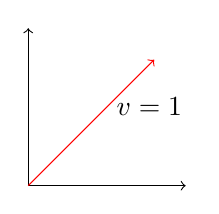
\begin{tikzpicture}[scale=2]
        \draw[->] (0,0) -- (0,1);
        \draw[->] (0,0) -- (1,0);
        \draw[->, red] (0,0) -- (0.8,0.8);
        \node[right] at (0.5,0.5) {$v=1$};
    \end{tikzpicture}
    \caption{World line of a photon}
    \label{PhotonWL}
\end{figure}

The transformation between coordinates in two inertial frames of an event $P$ is called a \emph{Lorentz transformation}. We begin with some ``standard configuration'' such that $x=y=z=t=0, x' = y' = z' = t' = 0$ but then have $S'$ frame move along the $+x$ axis with speed $v < 1$. Thus, the space-time diagram for the two frames looks like Figure \eqref{TwoWorld}
\begin{figure}[!h]
    \centering
    \begin{tikzpicture}[scale=2]
        \draw[<->] (-1,0) -- (1,0);
        \node[below] at (1,0) {$x$};
        \draw[<->] (0,-1) -- (0,1);
        \node[left] at (0,1) {$t$};
        \draw[<->] (-0.1,-1) -- (0.1,1);
        \node[right] at (0.1,1) {$t'$};
        \draw[<->, red] (-1,-0.1) -- (1,0.1);
        \node[above] at (1,0.1) {$x'$};
    \end{tikzpicture}
    \caption{The $x'$ axis is defined as the line of constant $t' = 0$.}
    \label{TwoWorld}
\end{figure}

How do we define the line of $t' = 0$? Consider a line that lies at constant $x'_0$. Consider a pulse starting at time $-\tau$ that starts at position $x'_1 \neq x'_0$ that heads towards the line. Suppose it bounces off this line and comes back to the starting $x'_1$ at exactly some time $\tau$. Then we know it must have hit $x'_0$ at $t'=0$! This is how we define this line. Let's then examine this event in the two frames using space-time diagrams (having fun with tikz) in Figures \eqref{BouncePrime} and \eqref{BounceUnPrime}.
\begin{figure}[!h]
    \centering
    \begin{tikzpicture}[scale=2]
        \draw[<->] (-1,0) -- (1,0);
        \node[below] at (1,0) {$x'$};
        \draw[<->] (0,-1) -- (0,1);
        \node[left] at (0,1) {$t'$};
        \draw[blue] (0,-0.5) -- (0.5,0);
        \draw[blue] (0,0.5) -- (0.5,0);
    \end{tikzpicture}
    \caption{The bounce in the primed frame.}
    \label{BouncePrime}
\end{figure}
\begin{figure}[!h]
    \centering
    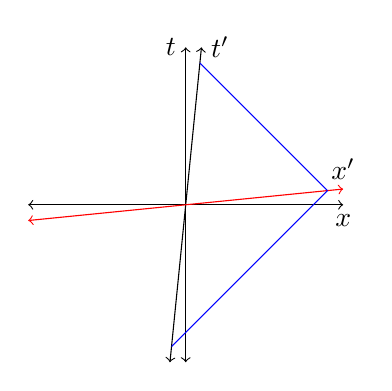
\begin{tikzpicture}[scale=2]
        \draw[<->] (-1,0) -- (1,0);
        \node[below] at (1,0) {$x$};
        \draw[<->] (0,-1) -- (0,1);
        \node[left] at (0,1) {$t$};
        \draw[<->] (-0.1,-1) -- (0.1,1);
        \node[right] at (0.1,1) {$t'$};
        \draw[<->, red] (-1,-0.1) -- (1,0.1);
        \node[above] at (1,0.1) {$x'$};
        \draw[blue] (-0.09, -0.9) -- (0.9,0.09);
        \draw[blue] (0.9,0.09) -- (0.09, 0.9);
    \end{tikzpicture}
    \caption{The bounce qualitatively in the unprimed frame. Note that both bounces have slope 1 still.}
    \label{BounceUnPrime}
\end{figure}

We then can set up the bounce to force the equations
\begin{align}
    x' &= \gamma(x-vt)\\
    t' &= \tilde{\gamma}(t-vx)\\
    x &= \gamma(x' + vt')\\
    t &= \tilde{\gamma}(t' + vx')
    \label{LorentzDeriv}
\end{align}

Checking these equations and substituting the second set into the first set, we find $\gamma = \tilde{\gamma} = \frac{1}{\sqrt{1-v^2}}$. We note that transverse coordinates must be unchanged, as this would violate relativity. This then gives the full Lorentz transformation
\begin{align}
    x' &= \gamma(x-vt) & x &= \gamma(x' + vt')\\
    t' &= \gamma(t-vx) & t &= \gamma(t' + vx')\\
    y' &= y & z' &= z
    \label{Lorentz}
\end{align}

Note that this reduces to the Galilean transformation for $\gamma = 1$ the nonrelativistic case. Let's try some examples so we learn to be careful. First, length contraction.

Suppose I have a ruler of rest length $l_r = 1$ yard that is comoving with $S'$. What is its length in $S$? First, we define the length to be the simultaneous distance between the two events that define the ends of the ruler, phew! We then define $l_v$ the contracted distance to be such that when we have one end at $x=0$ at $t=0$ and another end at $l_v, t=0$ in the $S$ frame. We then note that we have $x' = l_r$ while we don't know $t'$, so the correct equation to use is $x' = \gamma(x-vt)$ which yields $l_r = \gamma l_v$. It is then clear that $t' \neq 0$, and so $S'$ frame claims that the two events used to define the length of the ruler are not simultaneous.

Let's then investigate time dialation. Let's pick the clock at the space origin of the $S'$ frame. If we then examine at some time $\tau'$, we find that $x' = 0, t' = \tau'$ which yields that we want to compute using $t = \gamma(t' + vx') = \gamma \tau'$. This problem is tricky because it is not symmetric unlike the previous problem! Note that $\tau'$ is the time is the clock present at both events, starting at the origin and measured again after some time $\tau'$. However, $t$ is the time measured on the same ruler of clocks but with different clocks! So $\tau'$ is the smallest possible time that can be measured between two events and we call this time the \emph{proper time}. This is why particle lifetimes are so much longer than we expect! Their lifetime is the proper time, but their lifetime is dialated to us.

\chapter{1/9/14 - Geometric approach to relativity}

An alternative statement of the principle of relativity is that ``every law must be expressible as a geometric frame independent relationship between geometric, frame independent objects'' so vectors.

Consider Newtonian mechanics as a relation between vectors $\vec{F} = m\vec{a}$ and isotropicness of space. Let's then consider EM equation $\vec{\nabla} \times \vec{E} = -\pd{\vec{B}}{t}$. We recall that this is consistent with relativity by some bashiness (refer to Purcell for this), but we can do better by putting this in terms of frame independent objects as well! One sees the utility of this approach.

Events are the first and easiest frame independent quantities; all frames agree an event happened. Worldlines (set of events) are then obviously frame independent as well. We can take a look at the infamous twin paradox from here. Note that in any inertial frame the non-accelerating twin has a straight worldline and the rocket twin certainly does not, which disproves the apparent symmetry. We can sketch it in a particularly simple frame of reference namely the frame of the rest twin
\begin{figure}[!h]
    \centering
    \begin{tikzpicture}[scale=0.7]
        \draw[<->] (-5,0) -- (5,0);
        \node[right] at (5,0) {$x$};
        \draw[<->] (0,-5) -- (0,5);
        \node[above] at (0,5) {$y$};
        \draw[blue] (0,0) -- (0,4);
        \draw[blue, domain = 0:2] plot(\x, {2 + sqrt(2) * sqrt(-\x + 2)});
        \draw[blue, domain = 0:2] plot(\x, {2 - sqrt(2) * sqrt(-\x + 2)});
    \end{tikzpicture}
    \caption{Two worldlines of the twins}
    \label{1.9.twinsLine}
\end{figure}

Then the stationary twin measures the proper time and must measure the longest time.

Let's then consider the concepts of future/past with respect to frame independence. If two points $O, P$ are separated by a line of slope $\frac{\Delta x}{\Delta t} > 1$, then the two points cannot influence one another. If they did, we can construct a frame $S'$ such that $\Delta t' = \gamma \Delta t\left( 1 - v\frac{\Delta x}{\Delta t} \right)$ where $v$ is the speed of $S'$ such that $\Delta t' < 0$ and the order of events is reversed! Thus the two events cannot cause one another, because observers would disagree on which came first! Clear solution to the chicken/egg problem.

We can then introduce the concept of the light cone
\begin{figure}[!h]
    \centering
    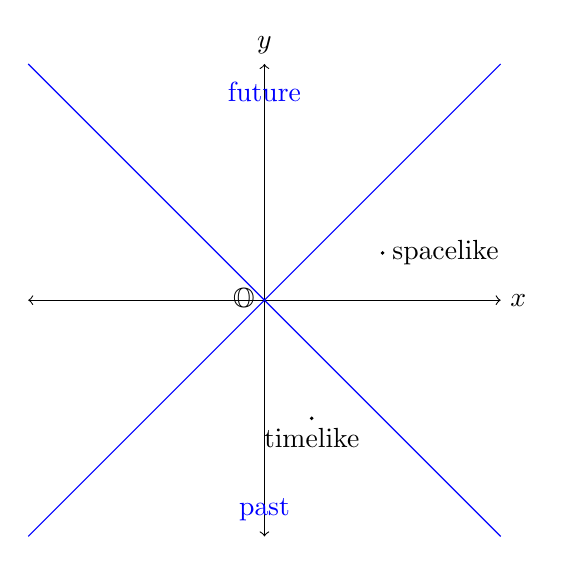
\begin{tikzpicture}[scale=0.3]
        \draw[<->] (-10,0) -- (10,0);
        \node[right] at (10,0) {$x$};
        \draw[<->] (0,-10) -- (0,10);
        \node[above] at (0,10) {$y$};
        \node[left] at (0,0) {$\mathbb{O}$};
        \node[blue, above] at (0,8) {future};
        \node[blue, below] at (0,-8) {past};
        \draw[blue] (-10,-10) -- (10,10);
        \draw[fill] (5,2) circle[radius=0.05];
        \node[right] at (5,2) {\text{spacelike}};
        \node[below] at (2,-5) {\text{timelike}};
        \draw[fill] (2,-5) circle[radius=0.05];
        \draw[blue] (-10,10) -- (10,-10);
    \end{tikzpicture}
    \caption{Light cone is between blue lines; defines causality and non-causality}
    \label{1.9.lightcone}
\end{figure}

We then see that past/future are frame independent objects. A fourth example of frame independent objects are 4-vectors which are straight lines joining two events. Suppose we have a 4-vector $\mathbf{\Delta x}= (\Delta t, \Delta \vec{x})$ in some frame $S$. Then in some frame $S'$ we know that it will have different coordinates related by a Lorentz transformation.

We wish then to define the magnitude of 4-vectors. For any timelike 4-vector $\mathbf{\Delta x}$ with magnitude $\Delta s^2$ we note that $\Delta s^2 = \Delta \tau^2$ where $\Delta \tau$ is the proper time between the two events (as a clock can be found such that it is present at both events). For any spacelike 4-vector it is possible to find a stationary ruler (in some frame of reference) such that the two events are simultaneous, and so $\Delta s^2 = - \Delta l^2$. For any event on the light cone it is evident that $\Delta s^2 = 0$, and so in the end we find that $\Delta s^2 = \Delta \tau^2 - \Delta x_1^2 - \Delta x_2^2 - \Delta x_3^2$. 

The dot product of two four vectors is given $\mathbf{\Delta x_1} \cdot \mathbf{\Delta x_2} = \Delta t_1\Delta t_2 - \Delta x_1 \Delta x_2 - \Delta y_1 \Delta y_2 - \Delta z_1\Delta z_2$. How do we construct 4-vectors? Of course we can scale a 4-vector by a constant. Otherwise, if an object $\mathbf{A}$ dots into an arbitrary 4-vector $\mathbf{B}$ to produce a Lorentz invariant scalar, then $\mathbf{A}$ is a 4-vector. Thirdly if components transform by a Lorentz transformation then it is a 4-vector.

Let's examine 4-velocity. Suppose we have two events on the worldline separated by 4-vector $d\mathbf{x}$. Then we define 4-velocity to be $\mathbf{u} = \rd{\mathbf{x}}{\tau}$ where $d\tau$ is the proper time separating the two events. In then the comoving frame we find $\mathbf{u} = (1,0,0,0), d\mathbf{x} = (d\tau, 0,0,0)$, and so most curiously $\mathbf{u}^2 = 1$. In a frame $S'$ in which the 3-velocity of the particle is $\vec{u}$, we can compute $u^0 = \rd{t}{\tau} = \gamma_u, u' = \rd{x}{\tau} = \rd{x}{t}\rd{t}{\tau} = \gamma_u u_x$ which shows that in $S'$ we have $\mathbf{u} = (\gamma_u, \gamma_u \vec{u})$ with $\gamma_u = \frac{1}{\sqrt{1-u^2}}$. 

We then note that frames are related to one another not by a velocity $\vec{v}$ but by a 4-vector $\mathbf{v}$. We can then either use Lorentz transforms of $\Delta x_i, \Delta t$ or properties of a 4-vector to write down the 3-velocity transformation rules
\begin{align*}
    u_x &= \frac{u_{x'} + v}{1+vu_{x'}}\\
    u_y &= \frac{u_{y'}}{1+vu_{x'}}\\
    u_z &= \frac{u_{z'}}{1+vu_{x'}}
\end{align*}

We can then look to the 4-momentum defined as $\mathbf{p} = m\mathbf{u}$ with $m$ the straight-up mass. Note then that $\mathbf{p}^2 = m^2$. Then in frame $S$ in which 3-velocity is $\vec{u}$ we have $\mathbf{p} \to (m\gamma_u, m\gamma_u \vec{u})$ which suggests that the relativistic 3-momentum is $m\gamma_u \vec{u}$. If we then examine the time-like component we find that expands to first order in $u$ to the Newtonian kinetic energy, so we suspect that the relativistic energy is the time-like component! Thus, $\mathbf{p} \to (E,\vec{p})$. We then can take the magnitude to find $(\mathbf{p})^2 = m^2 = E^2 - \vec{p}^2, E^2 = m^2 + p^2$.

We can then examine the 4-acceleration, namely $\mathbf{a} = \rd{\mathbf{u}}{\tau} = \left( \gamma^4\vec{u}\cdot \vec{a}, \gamma^2\vec{a} + \gamma^4(\vec{u\cdot\vec{a}}\vec{u} \right)$. It's a big mess, and so it suggests using $\vec{F} = m\vec{a}$ is not advisable!

We can lastly try to determine the concept of the gradient of a 4-vector. Suppose we have some $x' = x'(x,y,z,t)$, then by chain rule we can compute $\pd{}{x'} = \pd{x}{x'}\pd{}{x} + \pd{y}{x'}\pd{}{y} + \pd{z}{x'}\pd{}{z} + \pd{t}{x'}\pd{}{t}$ and since we can use Lorentz transform to compute the partials we have a gradient 4-vector $\mathbf{\nabla} = \left( \pd{}{t}, -\vec{\nabla} \right)$.

\chapter{1/14/14 - Relativistic Dynamics, 4-forces}

Recall that 4-momentum is defined $\mathbf{p} = m\mathbf{u} = (m\gamma_u, m\gamma_u \vec{u})$ with components relativistic energy and momentum. Useful expressions are that $E^2 = m^2 + p^2$, $\vec{u} = \frac{\vec{p}}{E}$.

Noting then that 4-momentum is a 4-vector, we can apply the Lorentz transformation to it via
\begin{align}
    p_x' &= \gamma(p_x - vE) & p_x &= \gamma(p_x' + vE')\\
    p_y' &= p_y & p_y &= p_y'\\
    p_z' &= p_z & p_z &= p_z'\\
    E' &= \gamma(E - vp_x) & E &= \gamma(E' + vp_x')
    \label{1.14.4pLorentz}
\end{align}

We will discuss relatistic collisions, forces/acceleration, and the Lagrangian approach.

Collisions are an important topic, i.e. particle physics. Collisions are classified as elastic (masses of particles unchanged) or inelastic (kinetic energy/masses are exchanged, maybe even new particles). 4-momentum is conserved in all collisions. General approach is to transform into frame where total 3-momentum is zero (center of mass), solve in this frame, and transform back.

One method is as follows. We begin by choosing the $x$ direction such that $p_y = p_z = 0$ and choose the $S'$ frame to be such that $p'_x = 0$, which yields the speed of $S'$ relative to $S$ to be $\frac{p_x}{E}$. We then transform energies/3-momenta to $S'$ using Lorentz transformations, solve in $S'$ and transform back to $S$

Another method is to use the invariance of scalar products $\mathbf{p}_a \cdot \mathbf{p}_b = \mathbf{p}_a' \cdot \mathbf{p}_b'$ with these two momenta any of the particle 4-momenta in the lab/CM frame. We must choose carefully though.

Consider Compton scattering, where some $\gamma$ ray is scattered off an electron. For now we will call the leaving $\gamma$ ray primed, so we want to find $E'_\gamma(\theta')$ the energy of the ray as a function of the scattering angle. We know then that 4-momentum is conserved $\mathbf{p}_\gamma + \mathbf{p}_e = \mathbf{p}_\gamma' + \mathbf{p}_e'$.

We know that $\mathbf{p}_e^2 = \mathbf{p}_e'^2 = m^2, \mathbf{p}_\gamma^2 = \mathbf{p}_\gamma'^2 = 0$. If we rewrite the conservation equation $\mathbf{p}_e' = \mathbf{p}_e + (\mathbf{p}_\gamma - \mathbf{p}_\gamma')$ (adding zero) and taking the dot product with itself we obtain
\begin{align}
    \mathbf{p}_e'^2 = m^2 &= \mathbf{p}_e^2 + 2\mathbf{p}_e(\mathbf{p}_\gamma - \mathbf{p}_\gamma') + \mathbf{p}_\gamma^2 + \mathbf{p}_\gamma'^2 - 2\mathbf{p}_\gamma\mathbf{p}_\gamma'\\
    0 &= 2m(E_\gamma - E_\gamma') - 2E_\gamma E_\gamma'(1-\underbrace{\hat{n}'\hat{x}}_{\cos \theta'})\\
    \frac{1}{E_\gamma'} - \frac{1}{E_\gamma} &= \frac{1}{m}\left(1 - \cos \theta'  \right)\\
    \lambda' - \lambda &= \frac{h}{mc}\left( 1-\cos\theta' \right)
    \label{1.14.scattering}
\end{align}
where we define $\hat{x}$ to be the direction of the initial $\gamma$ beam and $\hat{n}$ to be the direction of the $\gamma'$ beam. We also make in the last step substituitons $E_\gamma = \frac{hc}{\lambda}$. Note that QM is necessary to give us probabilty distribution of scattering at angle $\theta$.

Let's try an inelastic collision, colliding putty balls. Place one mass $b$ at rest and another mass $a$ moving to the right with 3-velocity $\vec{u}_a$. They will stick together and move with 3-velocity $\vec{u}$. Let's then consider the equation
\begin{align}
    m^2 = \mathbf{p}_{out}^2 = \mathbf{p}_{in}^2 &= \mathbf{p}_a^2 + \mathbf{p}_b^2 + 2\mathbf{p}_a\cdot \mathbf{p}_b\\
    &= m_a^2 + m_b^2 + 2m_bE_a \geq (m_a + m_b)^2\\
    \vec{u} = \frac{p_{out}}{E_{out}} = \frac{p_{in}}{E_{in}}&= \frac{\gamma_u m_a\vec{u}_a}{\gamma_a m_a + m_b}
    \label{1.14.putty}
\end{align}

Obviously the last equation is the one that is really key, we just demonstrate a counter-intuitive effect in the first result!

Let's then consider proton-antiproton production. We have a proton colliding with another proton at rest, and we ask what is minimum velocity such that two proton-antiproton pairs are produced. At the threshold, the four vector of the resulting pairs is $\mathbf{p} = (4m_p, \vec{0})$ which can be thought of as two pairs of particles with 4-momenta $(2m_p, \pm m_p)$. If we then compute invariant $\mathbf{p}_a \cdot \mathbf{p}_b = \mathbf{p}_a' \cdot \mathbf{p}_b'$ we obtain 
\begin{align}
    E_am_p &= 4m_p^2 + (p^*)^2\\
    &= 4m_p^2 + (4m_p^2 - m_p^2)\\
    &= 7m_p^2
\end{align}
which shows us that the incident proton must have total $7m_p$ energy, so $6m_p$ of kinetic energy to produce pairs.

There is a 4-force defined as $\mathbf{f} = \rd{\mathbf{p}}{\tau}$ with components $\left( \gamma_p \rd{E}{t}, \gamma_u \rd{\vec{p}}{t} \right)$ in inertial frame $S$. It is not used much though due to propagation of forces being limited by speed of light. It is much more convenient to define the relativistic 3-force $\vec{f} = \rd{\vec{p}}{t}$. Then we note that $\rd{E}{t} = \vec{f}\cdot \vec{u}$.

The acceleration is even more complicated, and usually isn't even parallel to the force, as $\vec{f} = \rd{}{t}(m\gamma_u \vec{u}) = \gamma_u^2(\vec{u}\cdot \vec{a})\vec{u} + \gamma_u m\vec{a}$. For forces perpendicular and parallel to $\vec{u}$ the result is slightly easier. We will discuss 4-acceleration more in PS2.

The Lagrangian approach in relativistic mechanics is only slightly different in that $S = \int L d\tau$ with $\tau$ proper time. We can deduce that $L = -m$ to be the only feasible Lagrangian (wow!) in proper time. The Lagrangian then for any general frame of reference is $-m\sqrt{1-u^2}$.

The only new Lorentz-invariant is proportional to $\mathbf{u}\cdot \mathbf{A}$ and this produces full Lagrangian in all inertial frames $L = -m\sqrt{1-u^2} - q\Phi(\vec{x},t) + q\vec{u}\cdot \vec{A}(\vec{x},t)$. 

\chapter{1/16/14 - Relativistic metric}

Frames of reference $S$ are defined in terms of 4 basis vectors $\mathbf{e}_i$ with $\mathbf{e}_0$ connecting $(1,0,0,0)$ to $(0,0,0,0)$ and the rest being just coordinate basis vectors. We note that $\abs{\mathbf{e}_0}^2 = 1, \abs{\mathbf{e}_i}^2 = -1$ with $i \neq 0$. These vectors are obviously orthogonal and so orthonormal with the catch that normality can equal $-1$. More precisely
\begin{equation}
    \mathbf{e}_\alpha\mathbf{e}_\beta = \underbrace{g_{\alpha,\beta}}_{\text{metric tensor}}, g = \begin{bmatrix} 1 & 0 & 0 & 0\\0 & -1 & 0 & 0\\0 & 0 & -1 & 0\\0 & 0 & 0 & -1 \end{bmatrix}
    \label{1.16.metric}
\end{equation}

Construct then contravariant quantity $x^\alpha$ by $\mathbf{x} = x^\alpha \mathbf{e}_\alpha$ using the summation convention (note that it makes no sense to sum over two down or two up indicies!). We can also define covariant $x_\alpha = \mathbf{x} \cdot \mathbf{e}_\alpha$. 

We can then relate $x_\alpha = g_{\alpha\beta}x^\beta$ which gives that $\{x_\alpha\} = \left( t,-x,-y,-z \right)$. Similarly we can take inverse of the above relation $x^\alpha = g^{\alpha\beta}x_\beta$ with $g^{\alpha\beta} = (g_{\alpha\beta})^{-1}$. Then we can think of $g_{\alpha\beta}$ as ``lowering the index'' from top to bottom index and vice versa. Then the scalar product $\mathbf{A}\cdot\mathbf{B}$ becomes $A^\alpha B_\alpha$. 

Let's then examine how this works in change of reference frames. The matrix elements are related by $\mathbf{e}\alpha = \mathbf{e}_\beta'\Lambda_\alpha^\beta$. We can then note $x'^\beta = \Lambda_\alpha^\beta x^\alpha$ while $x_\alpha = x_b' \Lambda_\alpha^\beta$.

Then in our standard configuration $S,S'$ moving relatively in $x$ direction the $\Lambda$ change of basis matrix looks like
\begin{equation}
    \Lambda = \begin{bmatrix} \gamma & -\gamma v & 0 & 0\\-\gamma v & \gamma & 0 & 0\\0 & 0 & 1 & 0\\0 & 0 & 0 & 1 \end{bmatrix} 
    \label{1.16.changeBasis}
\end{equation}

Then for a general direction of the ``boost velocity'' we can rotate to the standard configuration, boost, then rotate back; the resulting matrix is atrocious and can be found in lecture sldes. 

Then we can consider 4-tensors. Recall that an n-tensor is a linear function of $n$ vectors that gives a scalar. We know that our 4-vectors are rank 1 tensors. Our covariant/contravariant components are 4-vectors while the metric tensor which relates covariants to contravariants must be a rank 2 4-tensor. We then ask how 4-tensors transform, and we note simply that $T'^{\alpha\beta} = \Lambda_\mu^\alpha \Lambda_\nu^\beta T^{\mu\nu}, T_{\alpha\beta} = T^{\mu\nu}\Lambda_\mu^\alpha \Lambda_\nu^\beta$.

We use this formalism because EM field tensor is very convenient. Defined in component form by $F^{\alpha\beta} = \partial^\alpha \mathbf{A}^\beta - \partial^\beta \mathbf{A}^\alpha$ with $\partial^\alpha = \left( \pd{}{t}, -\nabla \right), \mathbf{A} = (\phi, \vec{A})$. We can work this out to get
\begin{equation}
    F^{\alpha\beta} = \begin{bmatrix} 0 & -E_x & -E_y & -E_z\\
    E_x & 0 & -B_z & B_y\\
E_y & B_z & 0 & -B_x\\
E_z & -B_y & B_x & 0\end{bmatrix} 
    \label{1.16.emtensor}
\end{equation}

We don't know immediately how EM fields transform, but since we know how 4-tensors transform we can write $F'^{uv} = \Lambda_\alpha^\mu \Lambda_\beta^\nu F^{\alpha\beta}$. The result is 
\begin{align}
    E_x' &= E_x & B_x' &= B_x\\
    E_y' &= \gamma(E_y - vB_z) & B_y' &= \gamma(B_y + vE_z)\\
    E_z' &= \gamma(E_z + vB_y) & B_z' &= \gamma(B_z - vE_y)
    \label{1.16.emtransform}
\end{align}

We can note two invariants $2(B^2 - E^2), -8\vec{E}\cdot \vec{B}$. Then, for example, if we are solving the problem of a charge in $\vec{B}\cdot \vec{E} = 0$ subject to $E^2 - B^2 < 0$, we may find our life easier to transform to the frame where $\vec{E}' = 0$; note we can't find a frame where $\vec{B}' = 0$ because then it would necessitate $E^2 < 0$ by our invariant $E'^2 - B'^2 < 0$. We accomplish this by going to frame moving with relative velocity $\frac{E}{B}$. Then in the $S'$ frame the particle just circular motion in $xy$ plane along with translation in the $z$ direction. Then in $S$ frame we can just transfor back to get our motion. 

The EM field tensor describes the Lorentz force well. Consider Minkowski force $\mathbf{f} = q\mathbf{F}\cdot \mathbf{u}$ with $\mathbf{u}$ the particle 4-velocity. The equation of motion is then $\rd{\mathbf{p}}{\tau} = q\mathbf{F}\cdot \mathbf{u}$. This is considered a covariant description. 

The geometric definition of the metric tensor is that $g(\mathbf{u}, \mathbf{v}) = \mathbf{u}\cdot \mathbf{v}$.

\chapter{1/21/14 - Nonlinear oscillators}

Poincar\'e discovered in his study of the 3-body Kepler problem that certain problems are chaotic, namely two properties (no analytic solution, small change in initial condition produces much difference?). We will approach chaos thorugh nonlinear oscillators instead of three-body problem. We will examine single driven harmonic oscillators (Hamiltonian/damped) and eventually coupled nonlinear Hamiltonian oscillators.

The simplest nonlinear oscillator is the pendulum! $V(q) \propto 1-\cos q$. Of course we will start by looking at small-angle $V \approx \frac{q^2}{2} + \frac{aq^4}{4}$, called the Duffing oscillator. The general equation of motion is then
\begin{equation}
    m\rd{q}{t} + \Gamma\rd{q}{t} + Kq + aq^3 = F\cos \omega_d t
    \label{1.21.duffingComplex}
\end{equation}

We define $\omega_0^2 = \frac{K}{m}, Q = \frac{m\omega_0}{\Gamma}, \alpha = \frac{a}{m\omega_0^2}, f = \frac{F}{m\omega_0^2}$ and scale our frequencies $\tilde{t} = \omega_0 t, \omega = \frac{\omega_d}{\omega_0}$ to obtain
\begin{equation}
    \ddot{q} + \frac{1}{Q}\dot{q} + q + \alpha q^3 = f\cos \omega \tilde{t}
    \label{1.21.duffing}
\end{equation}

We will now omit $\tilde{t} \to t$. Let's first examine undriven, undamped case. Method of quadratures can solve this since energy is conserved, but w]let's try with more advanced techniques. The EOM is $\ddot{q} + q + \alpha q^3 = 0$. We solve this via perturbation theory instead of quadratures (tr this on your own!), so assume $\alpha = \epsilon \ll 1$. The unperturbed system is simple. 

We then apply pert theory, specifically ``method of successive approximations'' which is to write solution $q(t) = q_0(t) + \epsilon^1(\dots) + \epsilon^2(\dots) + \dots$. We then substitute back into the EOM and collect orders in $\epsilon$. This gives
\begin{align}
    \ddot{q}_0 + q_0 &= 0 \Rightarrow q_0 = A\cos t\\
    \ddot{q}_1 + q_1 &= -q_0^3 = -A^3\cos^3t\\
    \ddot{q}_2 + q_2 &= 3q_0^2 q_1\\\
    \ddot{q}_k + q_k &= F_k(t)
\end{align}

Note that each order depends only on previous orders. We know then that the Green's function can be used to write $q_k = \displaystyle\int\limits_{0}^{t}\sin(t-t')F_k(t')\;dt'$. When we solve out then for $q_1(t) = A^3\left( \frac{-3}{8}t\sin t - \frac{1}{32}\cos t + \frac{1}{32}\cos 3t\right)$. Examine this first term; amplitude growing in time means that for $t > \frac{1}{\epsilon}, \epsilon q_1(t) \sim q_0(t)$ meaning our approximation is only valid at small times $t$. This term is called the ``secular term.''

Let's examine where the physics comes from. Well, $F_1(t) = -A_3\cos^3 = -A_3\left[ \frac{3}{4}\cos t + \frac{1}{4}\cos 3t \right]$ where the first term drives the system exactly at resonance! The resolution is that we must apply what is called \emph{Lindstedt-Poincar\'e perturbation theory}.

What we ignored in setting up our ansatz was that frequency may change, so we must expand $\omega(\epsilon) = 1 + \epsilon\omega_1 + \epsilon^2\omega_2 +\dots$. We first note that $\cos[(1+\epsilon\omega_1)t]$ is not close to our original ansatz $\cos t$ for all time. The easiest way to do this is to rescale $s = \omega t$ and write $q(s) = \epsilon^i q_i(s), \dot{q} = \omega q'$. Our EOM then becomes $\omega^2 q'' + q + \epsilon q^3 = 0$. Then applying successive approximations we obtain
\begin{align}
    q_0'' + q_0 &= 0 \Rightarrow q_0 = A\cos s\\
    q_1'' + q_1 &= -q_0^3 + 2q_0\omega_1 \\
    &= \left( 2A\omega_1 - \frac{3}{4}A^3 \right)\cos s - \frac{A^3}{4}\cos 3s
\end{align}

In order then to force the secular term to vanish, we require the term in parentheses vanish and obtain $\omega_1 = \frac{3}{8}A^2$. Then the first order equation becomes a linear harmonic oscillator with driving force $-\frac{A^3}{4}\cos 2s$ which we know the solution must be of form particular integral plus complementary function, in our case $q_1 = -\frac{A^2}{32}\left( \cos s - \cos 3s \right)$. This then yields full solution
\begin{align}
    \omega &= 1 + \frac{3}{8}\epsilon A^2 +\dots\\
    q &= A\left( 1-\frac{\epsilon A^2}{32} \right)\cos \omega t + \frac{\epsilon A^3}{32}\cos 3\omega t +\dots
    \label{1.21.LPapprox}
\end{align}

Note that the scale of the problem is $\epsilon A^2$ where if this term is small then our expansion holds. We also exhibit a 3rd harmonic of amplitude $\epsilon A^2$ relative to the ground harmonic oscillator and a correction of size $\epsilon A^2$ to the first-order term. At least we have a periodic solution now. 

The driven, damped case is then given on lecture slides. Basically we expect a periodic solution oscillating at frequency $\omega$, so we just want to calculate amplitude/phase. Introducing $\tau = \omega t$ we arrive at EOM $q'' + q = \left( 1-\frac{1}{\omega^2} \right)q - \frac{1}{\omega Q}q' - \frac{\alpha}{\omega^2}q^3 + \frac{f}{\omega^2}\cos \tau$ with all small terms on the right. We will then multiply the right hand by $\mu$ and at the end we set $\mu = 1$ ($\mu$ is intuitively a counter of how many times the small terms pop up). 

The hardest part of pert theory is to determine what we want to solve. We know that we expect a final solution in phase space where all trajectories tend towards one with frequency $\omega$. In the zeroth order we know all solutions go with frequency $\omega$ but there is no ``tending towards'' a trajectory. One of these zeroth order solutions must be be the unperturbed solution that corresponds to the final solution in perturbed phase space, so we find that solution and perturb it! 

This out of the way, we just expand our EOM in terms of $\mu$. At $\mu^0$ we have $q''_0 + q_0 = 0$ which yields solution $q_0 = \frac{1}{2}\left( Aj^{i\tau} + A^*e^{-i\tau} \right)$ with $A$ encapsulating both the phase and amplitude of oscillation. At $\mu^1$ we plug this soution back through the EOM and remove secular terms by setting the secular coefficients of $e^{i\tau}$ to zero, obtaining 
\begin{align}
    \left[ \left( 1-\frac{1}{\omega^2} \right) - \frac{i}{\omega Q} - \frac{3\alpha}{4\omega^2}\abs{A}^2 \right]A &= -\frac{f}{\omega^2}\\
    -\frac{f}{(\omega^2 - \omega_{NL}^2 - i\frac{\omega}{Q}} &= A
\end{align}

This is the usual resonance formula, except that we have amplitude dependent frequency $\omega_{NL} \approx 1+\frac{3}{8}\alpha \abs{A}^2$ from the undriven case (thankfully they are different else secular case!). Note that $\omega$ is the frequency of the drive while $\omega_{NL}$ is the frequency at which the drive is greatest. What is fairly useful to plot is $\frac{A^2}{Q^2 f^2}$ the \emph{gain}, which he shows in class with a Mathematica notebook. Bascially the gain looks like a falling-over Lorentzian, and the solution exhibits a multiplicity of solutions at certain frequencies!

We can briefly describe harmonic analysis. Exhibit EOM $\ddot{q} + q + \alpha q^3 = f\cos \omega t$ (undamped for simplicity). The basic idea is that if we know the solution must oscillate at $\omega$, we write ansatz $q(t) = \sum_n A_n(\omega) \cos n\omega t + B_n(\omega)\sin n\omega t$. By examining some symmetries we can show that $B_n = 0$ for undamped, $A_{2n} =0$ for even potential/odd force. Then if $\alpha$ is small we think that $A_n$ decrease (so that $\alpha \to 0$ goes back to intuitive limit). Then we can plug this through our EOM (? I think?) and obtain terms in $\cos \omega t, \cos 3\omega t, \dots$ each of which must have vanishing coefficients. We can always keep only up to linear $\alpha$ and up to $A_1$ and obtain some reasonable resonance curves. 
\chapter{1/23/14 - Parametric drive}

An interesting problem is the periodic variation of a parameter, where for example we move the pivot of the pendulum up and down periodically, or equivalently varying $g$ periodically. Another example is if we vary the length of the pendulum periodically. In general the equation must look like $\ddot{q} + \frac{g}{l}q = 0$ (or some constant driving force). We then note that $q=0$ will always remain a solution.

Another curious case that we will do is of a horizontal bar being stretched and pushed, i.e. Figure \eqref{1.23.bar}
\begin{figure}[!h]
    \centering
    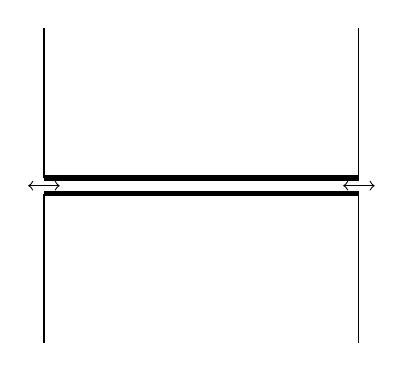
\begin{tikzpicture}[scale=0.5]
        \draw (-4,-4) -- (-4,-0.2);
        \draw (4,-4) -- (4,-0.2);
        \draw (4,4) -- (4,0.2);
        \draw (-4,4) -- (-4,0.2);
        \draw[<->] (-4.4,0) -- (-3.6,0);
        \draw[<->] (4.4,0) -- (3.6,0);
        \draw[line width=2pt] (-4, 0.2) -- (4,0.2);
        \draw[line width=2pt] (4, -0.2) -- (-4,-0.2);
    \end{tikzpicture}
    \caption{Picture of bar problem; bar can be pushed and pulled}
    \label{1.23.bar}
\end{figure}
Parametric drive in general is described by the Hill equation
\begin{equation}
    \ddot{q} + a(t)\dot{q} + b(t)q = 0
    \label{1.23.Hill}
\end{equation}

We know then Floquet's theorem, for a linear ODE with coefficients that are periodic with period $T$ solutions are of form $q(t) = e^{\sigma t}P(t)$ with $\sigma \in \mathbb{C}$ and $P(t)$ has period $T$. Note that $\Re\sigma$ plays the role of stability parameter; $\Re\sigma > 0$ produces unstable solution.

The general approach will be to solve for the first period $[0,T]$ and note that similar solution occurs in future periods, using the end conditions of the first period as initial conditions for the second period.. Secondly, since the Hill equation is linear in $q$ we can use superposition. The easiest way to use superposition is to solve for the two initial conditions $q(0) = 1, \dot{q} = 0$ or $q(0) = 0, \dot{q} = 1$, calling these two solutions $q_0, q_1$. The general solution is then given $q(t) = q(0)q_0 + \dot{q}(0)q_1$. Alternatively, we can write the \emph{monodromy matrix}
\begin{equation}
    \begin{pmatrix} q(T)\\ \dot{q}(T) \end{pmatrix} = \underbrace{\begin{pmatrix} q_0(T) & q_1(T)\\ \dot{q}_0(T) & \dot{q}_1(T) \end{pmatrix}}_{M}\begin{pmatrix} q(0)\\ \dot{q}(0) \end{pmatrix} 
    \label{1.23.monodromy}
\end{equation}

Then after $n$ periods $M$ the monodromy matrix must be exponentiated $n$ times and so it is convenient to go to the eigenbasis of $M$ assuming distinct eigenvalues. More precisely, we can write for eigenvectors $\vec{e}$
\begin{align}
    \begin{pmatrix} q(0)\\ \dot{q}(0) \end{pmatrix} = Q_i\vec{e}^i\\
    \begin{pmatrix} q(nT)\\ \dot{q}(nT \end{pmatrix} = \lambda_i^n Q_i \vec{e}^i\\
    \begin{pmatrix} q(nT + \tau)\\ \dot{q}(nT + \tau) \end{pmatrix} &= e^{\sigma_i (nT + \tau)}Q_ie^{-\sigma_i \tau}M\vec{e}^{i}
    \label{1.23.solHill}
\end{align}
We then know that if $\abs{\lambda} > 1$ then the corresponding solution has $\Re \sigma > 0$ giving instability.

Then for the Hamiltonian case, i.e. no dissipation we note that time evolution is a canonical transformation with generator Hamiltonian. Writing then $\dot{q} \to p$ we can write
\begin{align}
    \begin{pmatrix} q(T)\\ p(T) \end{pmatrix} = \bar{M}\begin{pmatrix} q(0)p(0) \end{pmatrix} 
\end{align}
with $\bar{M}$ the monodromy matrix, and then applying poisson brackets we see that $\det \bar{M} = 1$. This then says that the product of eigenvalues must be $1$, which means that computing the trace of $\bar{M}$ also gives us eigenvalues as $\mathrm{Tr} \bar{M} = \lambda + \frac{1}{\lambda}$. We note that these hold for the original monodromy matrix for position/velocity space since egienvalues are unchanged by change of coordinate basis. So writing $\lambda = \frac{1}{2}\mathrm{Tr} M + \sqrt{\left( \frac{1}{2}\mathrm{Tr} M \right)^2 - 1}$ we see that if $\abs{\mathrm{Tr}M} < 2$ then $\lambda$ is complex, $\abs{\lambda} = 1$ and we have oscillations at frequency different from drive frequency. Then if $\abs{\mathrm{Tr}M} > 2$ we have real eigenvalues and one must exceed $1$ which yields exponential growth.

Let's look at an example, a linear pendulum with a square wave driving force $\ddot{\theta} + \gamma\dot{\theta} + F(t)\theta = 0$ with $F(t)$ a square wave centered at $1$ with amplitude $r$ and period $T$. Then within each $T/2$ period we have just a constantly driven damped harmonic oscillator, and our $q_0, q_1$ initial conditions give us solutions
\begin{align}
    q_0 &= e^{-\gamma t/2}\left[ \cos \omega_{\pm}t + \frac{\gamma}{2\omega_{\pm}}\sin \omega_{\pm}t \right]\\
    q_1 &= e^{-\gamma t/2}\frac{1}{\omega_{\pm}}\sin_{\pm}t
    \label{1.23.squaresolutions}
\end{align}
with $\omega_{\pm}$ the appropriate frequencies of motion when solving the EOM (two roots to quadratic). We then construct our monodromy matrix and this yields the complete solution to our problem as a product of monodromy matricies during the up and down phases of the square wave. Then in the unstable equations we lose the linearity of the oscillator and we have to combine the equations of last lecture with this lecture to obtain the full solution.

Then with a harmonic drive we have $\ddot{\theta} + \gamma\dot{\theta} + \left[ 1 + h\cos \omega_0 t \right]\theta = 0$. We can then immediately drav the instability tongues, and we note that it is harder to excite the higher levels of instability in this case; we will not go through the actual solution. 

Since this is another resonance response phenomenon, it is very useful in amplifiers. 

\chapter{1/28/14 - Skipped: Introduction to chaos}

Note that time independent Hamiltonianss with a single DOF cannot give chaos since trajectories cannot cross and this restricts dynamics in phase space. We will thus examine the next simplest examples of chaos, 2 DOF and periodic $H$.

Let's do some examples before the theory. First, refer to double pendulum as canonical example of chaos. Let's then consider a rigid pendulum absent gravity, and we give it kicks $K\delta(t-n)\hat{x}$ at integer times. Dynamics can be considered by a discrete map $\theta_n, p_n$ as angle/momentum just after the $n$th kick. Note that between kicks $\theta_n$ evolves at rate $\dot{\theta} = p$ and $p$ stays constant while during kicks momentum changes while $\theta$ doesn't. This yields EOM
\begin{align}
    p_{n+1} - p_n &= K\sin\theta_{n+1}\\
    \theta_{n+1}-\theta_n &= p_n
    \label{1.28.EOM}
\end{align}

We usually transform by introducing $x_n = \frac{\theta_n}{2\pi} \mod 1, y_n = p_n$ to give \emph{standard map}
\begin{align}
    x_{n+1} &= x_n + \frac{y_n}{2\pi}\mod 1\\
    y_{n+1} &= y_n + K\sin\left( 2\pi x_{n+1} \right)
    \label{1.28.stdmap}
\end{align}

These standard maps can be examined numerically.

Let's first examine the concept of an integrable system; a system is \emph{integrable} if a canonical transformation to action angle variables exists. The action variables are then constants of motion and the angles evolve, so this is motion on an $N$-torus. What happens then when we introduce a perturbation?

The canonical transformation for $(\mathbf{q},\mathbf{p}) \to (\mathbf{\theta}, \mathbf{I})$ is solvable using Hamilton-Jacobi theory and canonical transformations, the zeroth order perturbation. Let's then express the perturbation in terms of the action angle variables of $H_0, H(I,\theta) = H_0(I) + \epsilon H_1(I,\theta)$. We then want to transform $H\to H'$ in new action angle variables $I', \theta'$.

We then do a lot of stuff in the lecture slides, but bottom line is that tori with rational relationship between action-angle frequencies will have their first-order perturbation diverge!

I don't understand his lecture notes. Refer to Ph106b Lecture 7 for more.
\chapter{2/4/14 - Dissipative Dynamical systems}

Skipped both chaos lectures, refer to notes.

Lorentz model is given
\begin{align}
    \dot{X} &= -\sigma(X-Y)\\
    \dot{Y} &= rX - Y - XZ\\
    \dot{Z} &= -bZ + XY
\end{align}

Computing phase space volume then $\nabla_{ph}\cdot \mathbf{V}_{ph} = -\sigma - 1 - b$ shows that phase space volumes contract uniformly and exponentially, characteristic of dissipative systems. Many systems then have \emph{attractors} that many/almost all initial conditions will tend to as transients die out, but since we don't have Hamiltonian formalism it is much more difficult to answer certain questions.

Let's start with one-dimensional system, $\dot{x} = f(x)$, which is already not doable in Hamiltonian formalism because Hamiltonian formalism requires $2n$ dimension phase space. Note that we can always turn an $n$-th order ODE into an $n$ dimensional system by ODE theory. We can then plot the flow either along the axis or plot $f(x)$ along the $x$ axis to show the direction of the flow. 

Suppose than we have $f(x) > 0 \forall x$, then $x$ will diverge to $\pm \infty$. We are normally interested in systems that don't diverge. The most physical system we can get is something like the $-\arctan(x)$ function, which is positive for $x < 0$ and negative for $x > 0$, exhibiting a stable fixed point at $x=0$. We note that the derivative at fixed points gives their stability, like ODEs. Then a condition for physical systems must be positive as $x \to -\infty$ and negative as $x \to \infty$. We then note that other than stable fixed points we expect alternating pairs of stable and unstable points. 

Bifurcations! These occur when a parameter is varied and fixed points are either added or removed. Bifurcations happen when a parabolic extremum is either pushed close to or taken away from $f(x) = 0$. For example, if we take a parabola $\dot{x} = x^2 - 1$ and push it to $\dot{x} = x^2 + 1$ near $x=0$ then we see that two fixed points vanish. In general, we can capture the qualitative aspects of the behavior using $\dot{x} = \mu + x^2$, the \emph{normal form} of the bifurcation, then $\mu$ is the bifurcation point. 

Plotting then the one-dimensional flow diagram as a function of $\mu$, we see that fixed point $x_0 = \pm \sqrt{-\mu}$ and only exist for negative $\mu$. The plot looks like
\begin{figure}[!h]
    \centering
    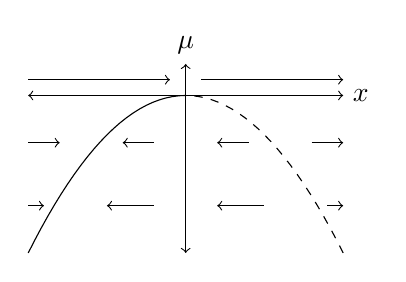
\begin{tikzpicture}[scale=0.2]
        \draw[<->] (-10,0) -- (10,0);
        \node[right] at (10,0) {$x$};
        \draw[<->] (0,-10) -- (0,2);
        \draw[->] (-10,1) -- (-1,1);
        \draw[->] (1,1) -- (10,1);
        \node[above] at (0,2) {$\mu$};
        \draw[domain=-10:0] plot(\x, \x^2/10);
        \draw[dashed, domain=10:0] plot(\x, -\x^2/10);
        \draw[->] (-10,-7) -- (-9,-7);
        \draw[->] (9,-7) -- (10,-7);
        \draw[<-] (-5,-7) -- (-2,-7);
        \draw[<-] (2,-7) -- (5,-7);
        \draw[->] (-10,-3) -- (-8,-3);
        \draw[->] (8,-3) -- (10,-3);
        \draw[<-] (-4,-3) -- (-2,-3);
        \draw[<-] (2,-3) -- (4,-3);
    \end{tikzpicture}
    \caption{Note the stable/unstable portions of the graph}
\end{figure}

This is called the bifurcation diagram, compact way to give stability at various parameters. This yields three results
\begin{itemize}
    \item One stable and unstable fixed point
    \item Separation of fixed points $\propto \sqrt{\abs{\mu}}$
    \item Stability eigenvalue is $0$ at the bifurcation. 
\end{itemize}

Instead of a stable and unstable point annihilating each other though, they could just pass through one another. We then fix one fixed point at the origin and obtain normal form $\dot{x} = \mu x - x^2$. Then we obtain the bifurcation diagram for the \emph{transcritical bifurcation}
\begin{figure}[!h]
    \centering
    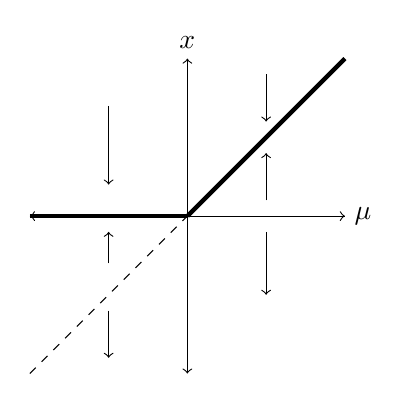
\begin{tikzpicture}[scale=0.2]
        \draw[<->] (-10,0) -- (10,0);
        \node[right] at (10,0) {$\mu$};
        \draw[<->] (0,-10) -- (0,10);
        \node[above] at (0,10) {$x$};
        \draw[ultra thick] (-10,0) -- (0,0);
        \draw[ultra thick] (0, 0) -- (10,10);
        \draw[->] (-5,7) -- (-5,2);
        \draw[->] (-5,-3) -- (-5,-1);
        \draw[->] (-5,-6) -- (-5,-9);
        \draw[->] (5,9) -- (5,6);
        \draw[->] (5,1) -- (5,4);
        \draw[->] (5,-1) -- (5,-5);
        \draw[dashed] (-10,-10) -- (0,0);
        \draw[dashed] (10,0) -- (0,0);
    \end{tikzpicture}
    \caption{Note the axes have flipped}
\end{figure}

Then we have what is called the pitchfork bifurcation which obeys normal form $\dot{x} = \mu x \pm x^3$ which occurs when the system has symmetry about $x \to -x$. Depending then on the sign we can have 
\begin{figure}[!h]
    \centering
    \begin{subfigure}{0.3\textwidth}
        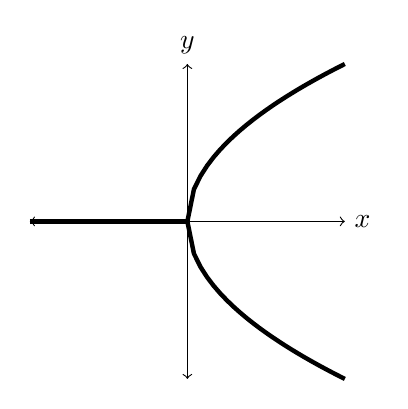
\begin{tikzpicture}[scale=0.2]
            \draw[<->] (-10,0) -- (10,0);
            \node[right] at (10,0) {$x$};
            \draw[<->] (0,-10) -- (0,10);
            \node[above] at (0,10) {$y$};
            \draw[ultra thick] (-10,0) -- (0,0);
            \draw[ultra thick, domain=0:10] plot(\x, {sqrt(10 * \x)});
            \draw[ultra thick, domain=0:10] plot(\x, {-sqrt(10 * \x)});
        \end{tikzpicture}
        \caption{Forward, supercritical}
    \end{subfigure}
    ~
    \begin{subfigure}{0.3\textwidth}
        \begin{tikzpicture}[scale=0.2]
            \draw[<->] (-10,0) -- (10,0);
            \node[right] at (10,0) {$x$};
            \draw[<->] (0,-10) -- (0,10);
            \node[above] at (0,10) {$y$};
            \draw[ultra thick, dashed] (10,0) -- (0,0);
            \draw[ultra thick, dashed, domain=0:-10] plot(\x, {sqrt(-10 * \x)});
            \draw[ultra thick, dashed, domain=0:-10] plot(\x, {-sqrt(-10 * \x)});
        \end{tikzpicture}
        \caption{backward, subcritical}
    \end{subfigure}
\end{figure}

In higher dimensional flows we can write normal form (choosing $x$ to be the direction in which the bifurcation happens)
$$\begin{cases} \dot{x} = \mu + x^2\\ \dot{y} = -y\end{cases}$$
where $\dot{y}$ is a fast contraction and $\dot{x}$ is a slow motion (we can choose these again, remember). Then we can have nodes and saddle points in the $x,y$ stream plot. 

But there arises a new bifurcation called the \emph{Hopf bifurcation} that arises for $n \geq 2$ dimensions. Let there be a fixed point at $x = y 0 $, and let's do stability analysis for $\delta \vec{x} = (\delta x, \delta y)$ and linearize about the fixed point, so
$$\delta \dot{\vec{x}} = \mathbf{J}\cdot \delta \vec{x}$$
where $\mathbf{J}_{ij} = \rd{f_i}{x_j}\Big|_{\vec{x} = 0}$ is the Jacobian. Then consider the eigenvalues of $\mathbf{J}$, either real or complex conjugates. Then as we vary $\mu$ one of the complex roots' real part will pass through $0$, which is the Hopf bifurcation as there will be an oscillation about the fixed point (imaginary part of the eigenvalue).

The normal form then, written in polar coordinates (most easily) is given
$$\begin{cases} \dot{r} = \mu r \mp r^3 \\ \dot{\theta} = w + br^2\end{cases}$$
and produces bifurcation diagram
\begin{figure}[!h]
    \centering
    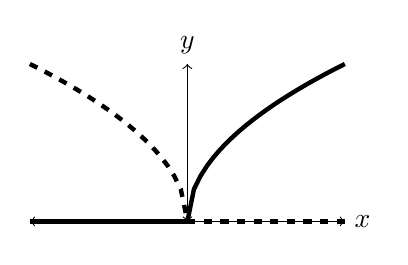
\begin{tikzpicture}[scale=0.2]
        \draw[<->] (-10,0) -- (10,0);
        \node[right] at (10,0) {$x$};
        \draw[<->] (0,0) -- (0,10);
        \node[above] at (0,10) {$y$};
        \draw[ultra thick] (-10,0) -- (0,0);
        \draw[ultra thick, dashed] (10,0) -- (0,0);
        \draw[ultra thick, domain=0:10] plot(\x, {sqrt(\x * 10)});
        \draw[ultra thick, dashed, domain=-10:0] plot(\x, {sqrt(\x * -10)});
    \end{tikzpicture}
    \caption{Hopf bifurcation diagram}
\end{figure}

Then if we want to examine limit cycles, we will want to examine the Poincar\'e section. We note that a limit cycle is then given by a fixed point on the Poincar\'e map, and so linear stability is determined by the eigenvalues of the Jacobian at the fixed points. 

\chapter{2/11/14 - Electrostatics introduction}

Electrostatics assumes that electric charges have been stationary forever and that the source charges are held fixed (no back reaction forces). We then start from Coulomb's Law
\begin{equation}
    \vec{F} = \frac{1}{4\pi \epsilon_0}\frac{qq'}{R^2}\hat{R}
\end{equation}
with $\vec{R} = \vec{r} - \vec{r}'$. $q,q'$ are in Coulombs and $\epsilon_0 = \scinot{8.85}{-12}\mathrm{C^2N^{-1}m^{-2}}$. The second principle we learned is the principle of superposition, where the force due to an ensemble of charges is the sum of the forces individually. 

Let's then look at continuous distributions of charge. The naive way to write this is $\vec{E} = \frac{1}{4\pi \epsilon_0}\int \frac{\hat{R}}{R^2}dq$. What does it mean then to integrate over a vector? Vector sum (or sum of the components along basis vectors). There are then three main configurations we see, line/surface/volume distributions. 

Let's then discuss the Dirac delta. Two properties, $\int_V f(\vec{r}) \delta(\vec{r} - \vec{r}_0) = 0, f(\vec{r}_0)$ depending on whether $\vec{r}_0 \in V$. Note the dimensions of the delta function are the reciprocal of its argument.

We can then notate an ensemble of point charges $\rho(\vec{r}) = q_i' \delta(\vec{r} - \vec{r}_i)$. 

Recall then Gauss's Law, with $\mathcal{F} = \oint_S\vec{E}\cdot d\hat{S} = \frac{1}{\epsilon_0}\int_V \rho dV$. We derive this, but the most curious fact is that $\frac{dA\hat{R}}{R^2}$ is the solid angle subtended by the $dA$ located at $\vec{r}_0$! 

We then note the differential version of Gauss's law, where when we apply divergence theorem to Gauss's Law out pops the differential form.

Let's prove the differential form directly (since now I'm paying attention). Consider
\begin{align}
    \vec{\nabla}\cdot \vec{E} &= \vec{\nabla}\cdot \frac{1}{4\pi \epsilon_0}\displaystyle\int\limits_{V'}^{}d\tau'\frac{\rho(\pvec{r})(\vec{r} - \pvec{r})}{\abs{\vec{r} - \vec{r}'}^3}\\
    &= \frac{1}{4\pi \epsilon_0}\displaystyle\int\limits_{V'}^{}d\tau' \rho(\vec{r}') \nabla \cdot \left( \frac{\vec{r} - \vec{r}'}{\abs{\vec{r} - \vec{r}'}^3} \right)
\end{align}
where we can pull the divergence (derivatives WRT $\vec{r}$) through the integral (WRT $\vec{r}'$). We then want some intuition as to what the divergence is, and since we struggle to do the integral directly we can look to the integral to tell us something about the function. We can apply divergence theorem to write then
\begin{align}
    \displaystyle\int\limits_{V}^{}\nabla \cdot \frac{\vec{r} - \vec{r}'}{\abs{\vec{r} - \vec{r}'}^3}\;d\tau' = \displaystyle\int\limits_{S}^{}da\hat{n}\cdot \frac{\vec{r} - \vec{r'}}{\abs{\vec{r} - \vec{r}'}^3}
\end{align}
which we then note that the right hand side is a solid angle so goes to $4\pi$ if $\vec{r}'$ is in $V$ and zero otherwise. Then we finish our proof easily.

We look back on our proof and note that at one step we had
\begin{align}
    \rho(\vec{r}) = \frac{1}{4\pi}\int d\tau' \rho(\vec{r}') \nabla\left( \frac{\vec{r} - \vec{r}'}{\abs{\vec{r} - \vec{r}'}^3} \right)
\end{align}
which is then obviously a delta function!

Let's then examine whether $\delta(\vec{r} - \vec{r}') = \delta(\vec{r}' - \vec{r})$? Consider the troll argument
\begin{equation}
    4\pi\delta(\vec{r} - \vec{r}') = \vec{\nabla}\cdot \frac{\vec{r} - \vec{r'}}{\abs{\vec{r} - \vec{r}'}^3} =- \vec{\nabla}\cdot \frac{\vec{r}' - \vec{r}}{\abs{\vec{r}' - \vec{r}}^3} = -4\pi \delta(\vec{r}' - \vec{r})
\end{equation}

The reason this is false is because the second $\vec{\nabla}$ is still taken WRT $\vec{r}$. Then consider that $\vec{\nabla}_{\vec{r}} = \vec{\nabla}_{\vec{r} - \vec{r}'}$, which is just an offset in the derivative! But then obviously $\vec{\nabla}_{\vec{r} - \vec{r}'} = -\vec{\nabla}_{\vec{r}' - \vec{r}}$ because we flip our axes, and then we see that $\vec{\nabla}_{\vec{r}} = -\vec{\nabla}_{\vec{r}'}$ and so plugging this through our troll proof we find that $\delta(\vec{r} - \vec{r}') = \delta(\vec{r}' -\vec{r})$ as expected.

\chapter{2/13/14 - Makeup: Potential (energy), conductors}

Key, curl of $\vec{E}$ always vanishes. We can see this by computing for arbitrary charge distribution
\begin{align}
    \curl\vec{E} &= \frac{1}{4\pi\epsilon_0} \curl \int_{\mathcal{V}}\rho(\vec{r}') \frac{\vec{r} - \vec{r}'}{\abs{\vec{r} - \vec{r}'}^3}d\vec{r}'\\
    &= \frac{1}{4\pi\epsilon_0} \int_{\mathcal{V}}\rho(\vec{r}') \curl\frac{\vec{r} - \vec{r}'}{\abs{\vec{r} - \vec{r}'}^3}d\vec{r}'
\end{align}

We note then $\vec{r}'$ is just an offset to $\vec{r}$, so if we define $\vec{s} = \vec{r} - \vec{r}'$ then we can try to show that $\curl \frac{\vec{s}}{s^3} = 0$, which given the symmetry is intuitively true. Refer then to Pg. 38 of lecture notes for the explicit formula for the curl, under which all derivatives vanish and $\curl \vec{E} = 0$.

Then Gauss's Law and the vanishing curl give information on the behavior of fields at boundaries. For example, to compute the change in normal component of electric field at an interface, we can draw a really stubby cylinder at the interface and find the relation between the charge density at the boundary and the change in electric field across the boundary. Similarly if we construct a loop normal to the surface and note that the line integral along the loop must vanish (Stoke's theorem and vanishing curl of $\vec{E}$) we can find that the tangential component of the electric field is continuous across any boundary.

In passing, we found that the line integral of the electric field along any closed loop $C$ vanishes. This implies that the electric field must be the gradient of a scalar potential, which we call the \emph{electric potential} defined $\vec{E}(r) = -\vec{\nabla}V(r)$ or 
$$V = \frac{1}{4\pi \epsilon_0}\displaystyle\int\limits_{\mathcal{V}}^{}\frac{\rho(\vec{r}')}{\abs{\vec{r} - \vec{r}'}}\;d\vec{r}^{\,\prime}$$

Note that the electric potential obeys superposition and is generally easier to work with than the vectors of the field.

We then can take note of \emph{Poisson's equation} $\nabla^2 V(\vec{r}) = -\frac{\rho(\vec{r})}{\epsilon_0}$, or when $\rho = 0$ we have the \emph{LAplace equation}.

We can also discuss the electrostatic energy of a configuration by noting that the work done going along a path is related to the line integral of the force/field along the line, and so it is natural to define the \emph{electric potential energy} $U = qV$. 

What then is the electric potential energy of some electrostatic configuration? Consider first the discrete case, bringing in each $i$th particle from infinity and summing the potential energy of the first $i-1$ charges, or
\begin{align}
    U_i &= \sum_{j=1}^{i-1}\frac{q_iq_j}{4\pi\epsilon_0\abs{\vec{r}_i - \vec{r}_j}}\\
    U &= \sum_{i=1}^{N}\sum_{j=1}^{i-1}\frac{q_iq_j}{4\pi\epsilon_0\abs{\vec{r}_i - \vec{r}_j}}\\
    &= \frac{1}{8\pi\epsilon_0}\sum_{i=1}^{N}\sum_{j=1, \neq i}^{N}\frac{q_iq_j}{\abs{\vec{r}_i - \vec{r}_j}}\\
    &= \frac{1}{8\pi\epsilon_0}\iint_\mathcal{V} \frac{\rho(\vec{r)}\rho(\vec{r}^{\,\prime})}{\abs{\vec{r} - \vec{r}^{\,\prime}}}\; d\vec{r}d\vec{r}^{\,\prime}
    \label{2.13.int}
\end{align}

Note that we omit the $i=j$ consideration in the integral formulation because while it explodes in the summation, it doesn't in the integration because $\rho(\vec{r}) \rho(\vec{r}^{\,\prime}) = 0$ as well. If we keep futzing with \eqref{2.13.int} a bit though, first using integration by parts then div theorem, we find
\begin{align}
    U &= \frac{1}{2}\int_\mathcal{V}\rho(\vec{r})V(\vec{r})d\vec{r} = -\frac{\epsilon_0}{2}\int_\mathcal{V}d\vec{r}\; V\nabla^2V\\
    &= -\frac{\epsilon_0}{2}\int_\mathcal{V} \div \left[ V\grad V \right]d\vec{r} + \frac{\epsilon_0}{2}\int_V\abs{\grad V}^2\;d\vec{r}\\
    &= \frac{\epsilon_0}{2}\int_\mathcal{S} d\vec{A} V\vec{E} + \frac{\epsilon_0}{2}\int_\mathcal{V}\abs{\grad V}^2\;d\vec{r}
\end{align}

Then let's think for a bit. $V,S$ are defined to enclose the entire charge distribution, but if we add a bunch of empty space over which there is no charge we can expect that $U$ doesn't change. Thus, let's define $V$ to be super big and therefore same with $S$. Then in this limit we note that the first integral vanishes and we obtain finally
\begin{equation}
    U = \frac{\epsilon_0}{2}\int\abs{\vec{E}(\vec{r})}^2\; d\vec{r}
\end{equation}

Careful, electric potential energy does not obey superposition! There are pairwise cross terms. 

We then talk a bit about conductors, where charges inside have complete mobility. They exhibit:
\begin{itemize}
    \item $\rho$ vanishes inside conductor.
    \item All charge lies on surface.
    \item Conductors are equipotential.
    \item Field just outside conductor is always normal.
\end{itemize}

If we then have conductors with cavity (and charge inside), we note that the charge inside the cavity is induced on the surface of the conductor.

Then we can define a \emph{capacitance} $C = \frac{Q}{\Delta V}$ between two conductors. We can generalize to multiple conductors by exhibiting $\vec{V}, \vec{Q}$ vectors and a capacitance matrix $\mathbf{C}, \vec{Q} = \mathbf{C}\vec{V}$. So for example in a configuration of two conductors with charge $\pm Q$ and voltage $\pm V$ we can compute
\begin{align}
    Q_1 &= 2CV = CV_1 - (-C) V_2\\
    Q_2 &= CV_2 - C V_1\\
    \mathbf{C} = \begin{bmatrix} C & -C\\-C & C \end{bmatrix} 
\end{align}

with $C$ our usual scalar capacitance. 

It should then be easy to see that to transmit some charge $Q$ across some capacitance $C$ we effectively store energy, and the age-old expression $U=\frac{Q^2}{2C}$ and friends. Then if we examine the multiple-capacitor case and do some summation voodoo algebra, we can find $U = \frac{\vec{Q}^{\,T}\mathbf{C}^{-1}\vec{Q}}{2}$ and friends (using expression $\vec{Q} = \mathbf{C}\vec{V}$).
\chapter{2/18/14 - Boundary Conditions, Method of images}

First we will discuss a few formal theorems. One result is for that of surface charge and force in a conductor. In a straight sheet then we have $\vec{E} = \frac{\sigma}{2\epsilon_0}\hat{n}$ pointing on both sides. Then if we are on a conductor the difference across the surface must be the same and so the field outside is $\frac{\sigma}{\epsilon_0}\hat{n}$. We can argue then that the force at each point on the conductor is given $\frac{\sigma^2}{2\epsilon_0}\hat{n} = \frac{\epsilon_0}{2}E^2\hat{n}$ by applying some boundary condition wizardry that is in lecture notes.

We then discuss capacitance very shortly. We know that $C = \frac{Q}{\Delta V}$. If we write the discretized case $V_i = D_{ij}Q_j$, this is just superposition of voltages! This is all in the notes so he's speeding really hard. We can also easily compute the potential energy of a set of conductors $U = \frac{q^2}{2C} = \frac{1}{2}\vec{Q}^{\,T}\mathbf{C}\vec{Q}$. 

Let's start the interactive portion of this class (new idea!). Suppose then we have a conductor of radius $R$ centered at the radius at the origin with charge $Q$, what are $C,U$? Hint: First relate $Q,V$ then compute $C$.

Yubo's try: We construct a Gaussian cylinder just outside $R$, then it is clear that $V = \frac{q}{4\pi\epsilon_0 R}$ after some careful work (uniform potential) relative to infinity. Then $C = \frac{Q}{V} = 4\pi\epsilon_0 R$. Then we can just apply $U = \frac{1}{2}\frac{Q^2}{C} = \frac{Q^2}{8\pi\epsilon_0R}$. 

Solution: Using Gauss's law we know that $\vec{E} = \frac{Q}{4\pi\epsilon_0}\frac{1}{r^2}\hat{r}$ which yields $V = \frac{Q}{4\pi\epsilon_0R}$. Then since $Q = CV$ we obtain $C = 4\pi\epsilon_0R$. Then plug through $U = \frac{Q^2}{2C} = \frac{Q^2}{8\pi\epsilon_0R}$. 

Let's then look to some uniqueness theorems. First, how do we solve the Laplace/Poisson equation? We already have an integral formulation for $V$ as a function of $\rho$ the charge density as the explicit solution to these equations, but a lot of the time we have a mix of voltages and charges; we don't easily know how to compute $\rho$. 

We examine this in more detail in 1D. The Laplace equation in 1D is $\rtd{V}{x} = 0$, so the general solution $V(x) = mx + b$. This then clearly exhibits an averaging property $V(x) = \frac{V(x+a) + V(x-a)}{2}$ and no relative extrema. Analogous properties in 3D Laplace equation $\nabla^2 V = 0$ include that the potential at any point is the average about some sphere about that point $V(\vec{r}) = \frac{\int da'V(\vec{r})}{\int da'}$ and that there are no relative extrema.

We can then look at Green's identities. First identity: $\oint_S \phi d\vec{A}\cdot \grad \psi = \int_V dV\left[ \psi\nabla^2 \phi + \grad \phi\grad \psi \right]$. The second identity, much more useful, is
\begin{equation}
    \oint_S da\left[ \phi\hat{n}\cdot \grad \psi - \psi\hat{n}\cdot \grad \phi \right] = \int_V dV\left[ \phi\nabla^2 \psi - \psi\nabla^2 \phi \right]
\end{equation}

We can then look at boundary conditions, fundamentally conditions that pin down the solution to the differential equations to a unique solution. The Dirichlet boundary condition is such that $V$ is specified everywhere on the surface of some volume $V$. The Neumann BC is when we instead specify $\hat{n}\cdot \grad V$, which is very similar to specifying $\sigma$ along a conductor (though keep in mind that this needn't be only for conductors). Of course there can be mixed BCs with some or another of the above two at every point.

Uniqueness then guarantees that given a complete set of BCs that our solution to Poisson's equation is unique. If $\mathcal{V}$ is surrounded by conductors on $S$ then solution is unique if $\rho$ inside $V$ is given and $Q$ on boundary is given.

Then we can look at the method of images. The idea is that if we can find an image charge distribution that matches the conductor boundary conditions then we can use the image instead, by uniqueness. Canonical example is a point charge and a conducting plate. Then if we compute the $V$ based on the images and plug through $\vec{E} = -\grad V, \sigma = \epsilon_0\rd{E}{z}$ we can find the induced $\sigma$. Note then that the charge is attracted to the conducting plate; how do we compute that force? Not by taking the grad of $V$, since this includes the charge's self-interaction! Instead we just compute the attractive force between images (I'm not gonna jot down the algebra since it's all in the lecture notes (LN)). Finally we compute the $U$ of the configuration. The foolproof way is to line-integral from infinity to the current configuration, careful about signs; answer is $U = -\frac{1}{4\pi\epsilon_0}\frac{q^2}{4d}$, negative as we expect. 

Let's set up one that is slightly more complicated. We have a point charge $q$ next to a conducting sphere, with the distance between the centers $a$ and spher radius $R$. Then we know our image charge must be on this axis, at some distance $b < R$ from the center of the sphere, nor do we know the magnitude $q'$ of the charge. What we do know however is that $V$ on the surface must be $0$, so we know that $V(a\pm R) = 0$ where $V = \frac{1}{4\pi\epsilon_0}\left[ \frac{q}{\abs{a-R}} + \frac{q'}{\abs{R-b}} \right]$; these are just the easiest BCs. One obtains $q' = -q\frac{R}{a}, b = \frac{R^2}{a}$.

Practice problem time! What is the force the point charge feels from the the induced charge density? Yubo thinks the easiest way to do this is to just compute the Coulomb force due to the point charge, but instructor tells us to compute the gradient of the non-self-interaction portion of the potential. Using my solution I obtain $\vec{E} = -\frac{qR}{4\pi\epsilon_0 a \abs{\vec{r} - \frac{R^2}{a}\hat{z}}}\hat{z}$. 

Solution: We want $\vec{E}(a\hat{z}) = -\hat{z}\grad \frac{q}{4\pi\epsilon_0}\frac{-\frac{R}{a}}{\abs{\vec{r} - \frac{R^2}{a}\hat{z}}}\Big|_{r = az}$. Computing this immediately at our point of interest $(0, 0, a)$ we finally obtain $\vec{E} = -\frac{q\frac{R}{a}}{4\pi\epsilon_0}\frac{1}{\left(a - \frac{r^2}{a}\right)^2}\hat{z}$. Additionally, it is clear that if we compute this just as the Coulomb force we will obtain the same answer (YES!).

If we then want the electrostatic potential energy we can then just take the line integral as we bring our point charge in from infinity. Keep in mind that if we want to compute the potential energy just as the potential energy between image charge and real charge we would again be off by some factor that again turns out to be $2$; I think he's trying to suggest that this factor isn't always $2$. We will discuss Green's functions on Thursday.
\chapter{2/20/14 - Makeup: Method of Green's Functions}

In the absence of a bounding surface (in the derivation we must take the volume/surface integral to infinity) we have the Green's function
\begin{equation}
    G(\vec{r}, \pvec{r}) = \frac{1}{4\pi\epsilon_0}\frac{1}{\abs{\vec{r} - \vec{r}'}}
\end{equation}

Then general source function $g(\vec{r})$ gives solution $V(\vec{r}) = \int d^3r' G(\vec{r}, \pvec{r}) \rho(\pvec{r})$.

Given more complex boundary condition Green's function requires a second term $F(\vec{r}, \pvec{r})$ with $\nabla^2_r F = 0$. We will discuss more on $F$ when we discuss other boundary conditions. 

If we apply the Green Function through Green's theorem we can find
\begin{align}
    V(\vec{r}) = \displaystyle\int\limits_{V}^{}dV\;\rho(\pvec{r})G(\vec{r}, \pvec{r}) + \epsilon_0\oint_S d\vec{A}\left[ G\cdot \grad_{r'}V(\pvec{r}) - V(\pvec{r})\cdot \grad_{r'} G \right]
\end{align}
which shows that once we know $G$ for one boundary condition and force the other boundary condition to vanish the general solution is just an integration over the source distribution and boundary condition. Let's show this with an example boundary condition\dots

Dirichlet boundary condition is just specifying $V$ on all boundary points. Since we only specify $V$ and not $\vec{\nabla}_{r'} V$ we should eliminate this from from our above. We can do this by requiring the Dirichlet Green Function $G_D(\vec{r}, \pvec{r}) = 0$ for $\pvec{r}\in S, \vec{r}\in V,S$. 
\begin{align}
    V(\vec{r}) = \displaystyle\int\limits_{V}^{}dV\;\rho(\pvec{r})G_D(\vec{r}, \pvec{r}) - \epsilon_0\oint_S d\vec{A}V(\pvec{r})\cdot \grad_{r'} G_D\label{Green.D}
\end{align}

Bunch of explanation about the intuition of Dirichlet BCs (refer to Jackson \S 1.8 --- 1.10). Next is Neumann boundary conditions, where $\div V$ is specified for $\vec{r}\in S$. The simplest condition we can impose is that
\begin{align}
    \hat{n} \cdot \div_{r'}G_N(\vec{r}, \pvec{r}) = -\frac{1}{\epsilon_0S}
\end{align}
with $S$ the surface area of our boundary. This gives us
\begin{align}
    V(\vec{r}) = \displaystyle\int\limits_{V}^{}dV\;\rho(\pvec{r})G_n(\vec{r}, \pvec{r}) + \epsilon_0\oint_S d\vec{A}\left[ G_n\cdot \grad_{r'}V(\pvec{r}) \expvalue{V} \right]
\end{align}

The appearance of the average potential term makes sense since under Neumann boundary conditions we can only specify the potential up to some offset.

We then recall how the Green's function has an offset term $F(\vec{r}, \pvec{r})$. We can determine it using the method of images often; consider two cases we have examined. First, point charge near conducting plane. We know the potential is given by the superposition of point charges, so we just let $dz = \pvec{r}$ and remove $q$ as follows
\begin{align}
    V(\vec{r}) &= \frac{1}{4\pi\epsilon_0}\left[ \frac{q}{\abs{\vec{r} - d\hat{z}}} - \frac{q}{\abs{\vec{r} + d\hat{z}}} \right]\\
    G_D(\vec{r}, \pvec{r}) &= \frac{1}{4\pi\epsilon_0}\left[ \frac{1}{\abs{\vec{r} - \pvec{r}}} - \underbrace{\frac{1}{\abs{\vec{r} + \pvec{r}}}}_{\propto F} \right]
\end{align}

We see that the second term accounts for the contribution from the induced charge by computing the effective potential. Note that the first term solves Poisson equation while second solves Laplace. Note also that the surface integral term that exists in Equation \eqref{Green.D} vanishes because $V(S) = 0$ (grounded).

We can also do the same example for a plate held at $V_0$ (hold infinity also at $V_0$). Intuitively we expect this should produce a constant potential offset in our Green Function. We can see this by noting that the surface integral (after pulling out the constant $V_0$) converges to the total image charge, which in our case is assumed to be $-1$ (negative of real charge) and so we obtain total contribution from surface integral $V_0$!

We also do an example with the point charge near a conducting sphere.

\chapter{2/25/14 - Separation of Variables}

Prereading: Separation of variables is powerful because it turns PDEs into ODEs. Then applying BCs we know from Sturm-Liouville theory that the set of solutions we find form a complete basis for all solutions to the BVP. Note also since the general Green's function solution comprises an inhomogeneous solution to Poisson's Equation $\frac{1}{4\pi\epsilon_0\abs{\vec{r} - \pvec{r}}}$ and homogeneous solution $F$ that satisfies the Laplace Equation for the BCs, we only need to develop separation of variables for the homogeneous solution, Laplace Equation solutions.

Assume $V(\vec{r}) = X(x)Y(y)Z(z)$, then plugging into Laplace Equation
\begin{align}
    \frac{1}{X}\rtd{X}{x} + \frac{1}{Y}\rtd{Y}{y} + \frac{1}{Z}\rtd{Z}{z} &= 0\\
\end{align}

This then shows that $\frac{1}{Q_i}\rtd{Q_i}{q_i} = C_i$ with the three constants summing to $0$. We know the general form of these solutions is exponentials $Q_i(q_i) = Ae^{q_i\sqrt{C_i}} + Be^{-q_i\sqrt{C_i}}$.

At this point we must proceed with examples. There are many in Griffiths, but one not in there is one with five sides of a box grounded and the other held at some potential $\phi(x,y)$, box side lengths $a,b,c$. This then yields boundary conditions
\begin{align}
    A+B &= 0 & Ae^{a\sqrt{C_1}} + Be^{-a\sqrt{C_1}} &= 0\\
    C+D &= 0 & Ce^{b\sqrt{C_2}} + De^{-b\sqrt{C_2}} &= 0\\
    A\left( e^{a\sqrt{C_1}}  - e^{-a\sqrt{C_1}} \right) &= 0\\
    C\left( e^{b\sqrt{C_2}} - e^{-b\sqrt{C_2}} \right) &= 0
\end{align}

This evidently only has solutions for oscillating exponentials, so we must take $C_1, C_2 < 0$. Then it becomes clear that the correct functional form (skipping a few obvious steps)
\begin{align}
    X(x) &= \sum_{n=1}^{\infty}A_n\sin \frac{n\pi x}{a}\\
    Y(y) &= \sum_{m=1}^{\infty}B_m\sin \frac{m\pi y}{b}
\end{align}

Easy enough. Let's do work on the last BC. We know already that 
\begin{align}
    Z(z) = E\exp\left( z\sqrt{-(C_1 + C_2)} \right) + F\exp\left( -z\sqrt{-\left( C_1 + C_2 \right)} \right)
\end{align}

We then know from BCs that $E=-F$ and that $C_i = \frac{n^2\pi^2}{a_i^2}$ (shorthand is getting a bit out of hand) so
\begin{align}
    Z(z) &= E\left[ \exp\left( z\sqrt{\frac{n^2\pi^2}{a^2} + \frac{m^2\pi^2}{b^2}} \right) - \exp\left( -z\sqrt{\frac{n^2\pi^2}{a^2} + \frac{m^2\pi^2}{b^2}} \right)\right]\\
    &= 2E\sinh(\gamma_{mn}z)
\end{align}
with $\gamma_{mn} = \sqrt{\frac{n^2\pi^2}{a^2} + \frac{m^2\pi^2}{b^2}}$. Note that we have yet to apply $\phi(x,y)$ BC.

We then impose the last BC. This takes on form (screw it, I'm using his notation $\alpha = \frac{n\pi}{a}, \beta = \frac{m\pi}{b}$)
\begin{align}
    \phi(x,y) &= \sum_{m,n = 1}^{\infty} A_{mn}\sin(\alpha_nx)\sin\left( \beta_my \right)\sinh(\gamma_{mn}c)
\end{align}

Using orthonormality then we know that
\begin{align}
    \displaystyle\int\limits_{0}^{a}\displaystyle\int\limits_{0}^{b}\phi(x,y)\frac{2}{\sqrt{ab}}\sin (\alpha_p x)\sin(\beta_q y)\;dxdy &= \frac{\sqrt{ab}}{2}A_{pq}\sinh(\gamma_{pq}c)
\end{align}

Note that this is just an application of orthonormality of $\sqrt{\frac{2}{a_i}}\sin \alpha_i q_i$. We can then write a really ugly formula for $V(\vec{r})$ that is in the notes.

Note that if we had a box with arbitrary potentials on all six surfaces, we can just superimpose six of the above solutions since each solution does not affect the boundary conditions of other solutions so the superposition satisfies all six arbitrary potentials. Most cases we will have to do this since separation of variables usually isn't guaranteed to work. 

Note then that when we compare our full solution to \eqref{Green.D} we can find an expression for the integrand of the surface integral easily. However, note that our solution \emph{does not} fully specify $F$. To fully specify $F$ we must use method of images with $V=0$ on all surfaces. This is much more guesswork however, and separation of variables is more reliable. Note also that method of images cannot solve for a Neumann boundary condition since method of images assumes $V=0$ a Dirichlet boundary condition.

Oops, didn't end up going to class. Let's just get some notes down really quickly.

Spherical coordinates separation of variables goes by making ansatz $V(r,\theta,\phi)$ is separable, resulting in equations
\begin{align}
    \frac{1}{\Phi(\phi)}\rtd{\Phi}{\phi} &= -m^2\\
    \frac{1}{R(r)}\rd{}{r}\left( r^2 \rd{R}{r} \right) &= l(l+1)\\
    \frac{1}{\Theta(\theta)}\frac{1}{\sin\theta}\rd{}{\theta}\left( \sin\theta \rd{\Theta}{\theta} \right)- \frac{m^2}{\sin^2\theta} &= -l(l+1)
\end{align}
producing solutions of form
\begin{align}
    \Phi(\phi) &= Ae^{im\phi} + Be^{-im\phi}\\
    R(r) &= Ar^{l} + \frac{B}{r^{l+1}}\\
    \Theta(\theta) &= P_l(\cos\theta)
\end{align}
the Legendre polynomials (derivation is in the notes, page 140ish.

Let's then assume azimuthal symmetry, in which case the potential must take on form
\begin{align}
    V(r,\theta) = \sum_{l=0}^{\infty}\left( A_lr^l + \frac{B_l}{r^{l+1}} \right)P_l(\cos\theta)
\end{align}

That's in for this lecture! I missed some examples probably, and I'm leaving out some algebra. Oops.
\chapter{2/27/14 - Spherical separation of variables, azimuthal symmetry and not}

\textbf{Note to self}: There must be a minimum of two BCs to pinpoint a solution to Laplace equation in each region, so per $n$ boundaries we need $n+2$ BCs to uniquely determine the solution.

Recall that in the case of separation of variables in spheriacl coordinates with azimuthal symmetry we showed that we can write our general solution to Laplace equation as
\begin{align}
    V\vec{r} &= \sum_{l=0}^{\infty}\left( A_l r^l + \frac{B_l}{r^{l+1}} \right)P_l(\cos\theta)
\end{align}

Let's try an example. Given $V(R,\theta)$ on a sphere of radius $R$ find $V(r,\theta)$ inside and outside the sphere. We will just solve $r < R$, as $r > R$ follows similarly.

If we are including the origin we note that the $\frac{B_l}{r^{l+1}}$ term can't be part of our solution, as it diverges $r \to 0$ but with no point charge at origin we cannot have this divergence. Thus $B_l \to 0$. (Note: if there were a point charge at the origin we must consider the $B_l$ case for $l = 0$ as the potential goes with $\frac{1}{r}$; the $B_l$ coefficients are usually used for some domain $r \neq 0$)

We also know the other boundary condition $V(R,\theta) = \sum_{l=0}^{\infty}A_lR^lP_l(\cos\theta)$. To find the $A_l$ we use the orthonormality of the $\sqrt{\frac{2l+1}{2}}P_l$ by integrating
\begin{align}
    \frac{2l+1}{2}\displaystyle\int\limits_{-1}^{1}V(R,\theta)\;d(\cos\theta) &= A_lR^l\\
    A_l &= \frac{2l+1}{2R^l}\displaystyle\int\limits_{-1}^{1}V(R,\theta)\;d(\cos\theta)
\end{align}

Then since we've determined $A_l$ coefficients we have the full $V(\vec{r})$ solution for $r < R$! This is analogous to the cartesian case where we use orthonormality instead of the trig functions.

For $r > R$ we have two BCs again, $V(r \to \infty) = 0, V(R, \theta)$. This shows that $A_l$ are zero, and the solution end sup
\begin{align}
    B_l &= \frac{2l+1}{2}R^{l+1}\displaystyle\int\limits_{-1}^{1}V(R,\theta)\;d(\cos\theta)
\end{align}

A few other examples in Griffiths that we can look into (broadly) are given. First, specify $\sigma(R,\theta)$ on the sphere. This is a Neumann boundary condition then because it gives the change in $\hat{n} \cdot \div V$ at $r = R$. Note this isn't a complete Neumann boundary condition though, because we are only given the charge $\frac{\sigma}{\epsilon_0} = \text{change in} \hat{n}\cdot \div V$. The other BCs are that $r > R$ needs $V(r \to \infty)\to 0$ and $r < R$ needs $V(r \to 0) < \infty$. Note again that the $V(\vec{r})$ is different on inside/outside of the sphere and the BCs allow us to solve for the two sets of $A_l, B_l$. We won't do this, but it's in Griffiths.

Another example is an uncharged metal sphere of radius $R$ in uniform $\vec{E} = E_0\hat{z}$. The BCs again are expectedly neither Neumann or Dirichlet. One is that $V(R,\theta)$ is constant. Another, since for $z \to \pm \infty$ the potential explodes, we can expect by symmetry that $V(z=0) = 0$. Third BC is that $V(r \to \infty)$ explodes with $E_0z = E_0r\cos\theta = E_0rP_1(\cos\theta)$. Thus, we expect only an $r=1$ term in the summation, so the general form should take on form $A_1r^1 + \frac{B_1}{r^2}$. The exact solution is $V(\vec{r}) = E_0\left( r-\frac{R^3}{r^2} \right)\cos\theta$ which turns out to be just the sum of the uniform field and the induced dipole field! 

Useful expansion
\begin{align}
    \frac{1}{\abs{\vec{r} - \pvec{r}}} &= \sum_{l=0}^{\infty}\frac{r^l}{R^{l+1}}P_l(\cos\theta)\label{2.27.useful}
\end{align}
with $r,R$ the min/max of $r, r'$ respectively.

Let's now move on to an interesting problem, but it's still an old problem! Point charge $a$ away from grounded sphere of radius $R$. What then is $V(r > R, \theta)$. We note that Laplace's equation is satisfied for $r \neq a$, so there must be a BC to force the two solutions to match up. We can write cleverly then
\begin{align}
    \sigma_a(\theta,\phi) &= \frac{q}{2\pi a^2\sin\theta}\delta(\theta) = \frac{q}{2\pi a^2}\delta(\cos\theta - 1)
\end{align}
to describe the point charge! If we integrate then $a^2d\Omega$ we recover $q$ so our clever writing works. Then noting that there are two regions of solution $r \in [R, a], r > a$ where both $A_l, B_l$ live inside while only the $B_l$ terms live outside, we will call the coefficient for the $r > a$ case $C_l$; notation will be clear in the equations.

First we solve for $r \in [R,a]$. Our first BC is $0 = V(R,\theta) = \sum_{l=0}^{\infty}A_lR^l + \frac{B_l}{R^{l+1}}P_l(\cos\theta)$ which then must vanish term by term so $A_lR^l = \frac{-B_l}{R^{l+1}}$. We can then rewrite $V(r,\theta) = \sum_{l=0}^{\infty}A_l\left( r^l - \frac{R^{2l+1}}{r^{l+1}} \right)P_l\cos\theta, r \in [R,a]$. Our second BC is that the two potentials must be continuous at $r=a$ which then yields $C_l = A_l\left( a^{2l+1} - R^{2l+1} \right)$ (similar math to above). The third BC is that $\rd{V}{r}\Big|_{r = a^+} - \rd{V}{r}\Big|_{r = a^-} = \frac{\sigma}{\epsilon_0}$ which is requiring that $\vec{E}$ changes by $\frac{\sigma}{\epsilon_0}$. Mathing pretty hard (he leaves this out in lecture too) we get 
\begin{align}
    -\sum_{l}^{}(2l+1)A_la^{l-1}P_l(\cos\theta) &= -\frac{q\delta(\theta)}{2\pi a^2\epsilon_0\sin\theta}
\end{align}

Then we use the same orthonormality trick of the $P_l$ to obtain the $A_l$ which is
\begin{align}
    -2\pi A_{l'}a^{l' - 1} &= -\frac{q}{2\pi a^2\epsilon_0} \displaystyle\int\limits_{0}^{\infty}\sin\theta\;d\theta\displaystyle\int\limits_{0}^{2\pi}d\phi\;\frac{\delta(\theta)P_{l'}(\cos\theta)}{\sin\theta}a^2\\
    &= -\frac{q}{\epsilon_0}\\
    A_l &= \frac{1}{a^{l+1}}\frac{q}{4\pi\epsilon_0}
\end{align}

Then we can write out our bitch of a solution explicitly
\begin{align}
    V(r < a, \theta) &= \frac{q}{4\pi\epsilon_0}\sum_{l=0}^{\infty}\left( \frac{r^l}{a^{l+1}} - \frac{\left( \frac{R}{a} \right)\left( \frac{R^2}{a} \right)^l}{r^{l+1}} \right)P_l(\cos\theta)\\
    V(r > a, \theta) &= \frac{q}{4\pi\epsilon_0}\sum_{l=0}^{\infty}\left( \frac{a^l}{r^{l+1}} - \frac{\frac{R}{a}\left( \frac{R^2}{a} \right)^l}{r^{l+1}} \right)P_l(\cos\theta)
\end{align}

Then if we recall \eqref{2.27.useful} we will obtain
\begin{align}
    V(\vec{r}) &= \frac{q}{4\pi\epsilon_0}\left[ \frac{1}{\abs{\vec{r} - a\hat{z}}} - \frac{R/a}{\abs{\vec{r} - \frac{R^2}{a}\hat{z}}} \right]
\end{align}

Let's now examine the case without $\phi$ symmetry. Recall then that the full solution includes a $\Phi(\phi) = Ae^{im\phi} + Be^{-im\phi}$ and the associated Legendre polynomials
\begin{align}
    P_l^m(x) &= (-1)^m(1-x^2)^{m/2}\left( \rd{}{x} \right)^mP_l(x)\\
    P_l^m(x) &= \frac{(-1)^m}{2^ll!}(1-x^2)^{m/2} \left( \rd{}{x} \right)^{l+m}\left( x^2-1 \right)l
\end{align}
with the second equation just the generalization of \emph{Rodruiguez's Formula} to the associated ones. Then allowing for an arbitrary dependence on $\phi$ we introduce the spherical harmonics
\begin{align}
    Y_{lm}(\theta, \phi) &= \sqrt{\frac{2l+1}{4\pi}\frac{(l-m)!}{(l+m)!}}P_l^m(\cos\theta)e^{im\phi}
\end{align}
for $l \geq 0, m \in [-l, l]$. Useful properties
\begin{itemize}
    \item $Y_{l(-m)} = (-1)^mY_{lm}^*$
    \item $\int d\Omega\; Y_{lm}^*Y_{l'm'} = \delta_{ll'}\delta_{mm'}$
    \item Completeness: $\sum_{l=0}^{\infty}\sum_{m=-l}^{l}Y_{lm}^*(\theta,\phi)Y_{lm}(\theta', \phi') = \delta(\phi - \phi')\delta(\cos\theta - \cos\theta')$
    \item $Y_l^0 = \sqrt{\frac{2l+1}{4\pi}}P_l(\cos\theta)$
    \item $P_l^{m\neq 0}(\pm 1) = 0, Y_{lm\neq 0}(0,\phi) = 0, Y_{l0}(0,\phi) = \sqrt{\frac{2l+1}{4\pi}}, Y_{l0}(\pi,\phi) = \left( -1 \right)^{-l}\sqrt{\frac{2l+1}{4\pi}}$
    \item Addition theorem $P_l(\hat{r}\cdot\hat{r}') = \frac{4\pi}{2l+1}\sum_{l=0}^{\infty}\sum_{m=-l}^{l}Y_{lm}^*(\theta', \phi')Y_{lm}(\theta,\phi)$
    \item Extension of \eqref{2.27.useful} to
        \begin{equation}
            \frac{1}{\abs{\vec{r} - \pvec{r}}} = 4\pi\sum_{l=0}^{\infty}\sum_{m=-l}^{l}\frac{1}{2l+1}\frac{r^l}{R^{l+1}}Y_{lm}^*(\theta', \phi')Y_{lm}(\theta,\phi)
            \label{2.27.useful2}
        \end{equation}
    \item General solutions to Laplace's equation are given $V(\vec{r}) = \sum_{l=0}^{\infty}\sum_{m=-l}^{l}\left( A_{lm}r^l + \frac{B_{lm}}{r^{l+1}} \right)Y_{lm}(\theta,\phi)$
    \item $\nabla^2 Y_{lm} = -\frac{l(l+1)}{r^2}Y_{lm}$
\end{itemize}

Let's now get to using some of these properties\dots Let's try to get the Green Function for grounded conducting sphere (best bud). We will just reexpress our Green Function using spherical harmonics
\begin{align}
    G_D(\vec{r}, \pvec{r}) &= \frac{1}{4\pi\epsilon_0}\left[ \frac{1}{\abs{\vec{r} - \pvec{r}}} - \frac{R/r'}{\abs{\vec{r} - \frac{R^2}{(r')^2}}\pvec{r}} \right]\\
    &= \frac{1}{\epsilon_0}\sum_{l=0}^{\infty}\sum_{m=-l}^{l}\left[ \frac{r_<^l}{r_>^{l+1}} - \frac{R}{r'}\frac{\left[ \frac{R^2}{r'}\right]^l}{r^{l+1}} \right]\frac{Y_{lm}^*(\theta',\phi')Y_{lm}(\theta,\phi)}{2l+1}
\end{align}
with $r_>, r_<$ the max and min of $r',r$ respectively. This can be useful even in spite of its ugliness, suppose for a charge distribution that is sinusoidal in $\phi$. 

Let's try to find the GF (Green Function) for \emph{even more general} (?? FML) case. Let's find it for arbitrary BC. We know that the general GF satisfies
\begin{align}
    -\epsilon_0 \nabla^2_{\vec{r}}G(\vec{r}, \pvec{r}) &= \delta(\vec{r} - \pvec{r})\\
    G(\vec{r}, \pvec{r}) &= \sum_{l=0}^{\infty}\sum_{m=-l}^{l}A_{lm}(r, \pvec{r})Y_{lm}(\theta,\phi)
\end{align}
where we just express $G$ as some arbitrary function for now. We then aim to expand the delta function to match coefficients
\begin{align}
    \delta(\vec{r} - \pvec{r}) &= \frac{\delta(r-r')}{r^2}\underbrace{\delta(\phi -\phi') \delta(\cos\theta - \cos\theta')}_{\sum Y_{lm} Y_{lm}}\\
    -\epsilon_0 \nabla^2 \sum_{l,m}^{}A_{lm}(r, \pvec{r}) Y_{lm}(\theta,\phi) &= \frac{\delta(r-r')}{r^2}\sum_{lm}^{}Y_{lm}^*(\theta', \phi')Y_{lm}(\theta,\phi)\\
    -\epsilon_0\sum_{lm}^{}\left[ \left( \nabla^2  - \frac{l(l+1)}{r^2} \right)A_{lm}(r, \pvec{r}) \right]Y_{lm} &=
\end{align}

Assuming then form $A_{lm}(r, \pvec{r}) = g_l(r, r')Y_{lm}^*(\theta', \phi')$ (note that the $\nabla^2$ doesn't act on $A_{lm}$ because it is WRT $r$ not $r'$) we match coefficients and obtain
\begin{align}
    -\epsilon_0\left( \nabla^2 -\frac{l(l+1)}{r^2} \right)g_l(r,r') &= \frac{\delta(r-r')}{r^2}
\end{align}

Then since the angular dependence has vanished we rewrite $\nabla^2 = \left( \rd{}{r} \right)^2$. This then is the radial equation from the Laplace equation!
\chapter{3/4/14 - Finsihing spherical Green Function, Multipole Expansion}

Pre-reading: The effect of the Green function is to embed some integrals into the solution so we don't have to do them anymore. With this in mind, it helps to express the Green function in terms of the $Y_{lm}$ (as we did before) to simplify some integrals when we integrate over charge symmetry, particularly when the distribution has some sort of symmetry (azimuthal). 

For our problems we will consider charge distributions inside a conducting sphere for which we use Green Function (from Jackson)
\begin{equation}
    G_D(\vec{r}, \pvec{r}) = \frac{1}{\epsilon_0} \sum_{l=0}^{\infty}\sum_{m=-l}^{l} r^l_< \left[ \frac{1}{r_>^{l+1}} - \frac{1}{b}\left( \frac{r_>}{b^2} \right)l \right]\frac{Y_{lm}^*(\theta', \phi')Y_{lm}(\theta,\phi)}{2l+1}
\end{equation}

Let's then examine as an example the potential inside the conducting sphere of radius $b$ due to an arbitrary Dirichlet boundary condition. We then need only to compute using \eqref{Green.D}, and since there is no enclosed charge we just need to compute the integrand of the surface integral. This is then
\begin{align}
    \hat{n}(\pvec{r})\cdot \grad_{\pvec{r}}G_D(\vec{r}, \pvec{r}) &= \frac{1}{\epsilon_0}\sum_{l,m}^{}\frac{Y_{lm}^*(\theta', \phi')Y_{lm}(\theta,\phi)}{2l+1}r^l \rd{}{r'}\left[ \frac{1}{(r')^{l+1}}- \frac{1}{b}\left( \frac{r'}{b^2} \right)^l \right]_{r' = b}
\end{align}
where we note we only want the radial component of the gradient. Evaluating this yields
\begin{align}
    \hat{n}(\pvec{r})\cdot \grad_{\pvec{r}}G_D(\vec{r}, \pvec{r}) &= -\frac{1}{\epsilon_0b^2}\sum_{l,m}^{}\frac{Y_{lm}^*(\theta', \phi')Y_{lm}(\theta,\phi)}{2l+1}r^l \left( \frac{r}{b} \right)^l
\end{align}
yielding potential
\begin{align}
    V(\vec{r}) &= \sum_{l,m}^{}\left( \frac{r}{b} \right)^lY_{lm}(\theta,\phi)\int d\Omega'\; Y_{lm}^*(\theta', \phi')V(b, \theta', \phi')
\end{align}

We note then that the spherical harmonic component of $V$ is related to the spherical harmonic component \emph{on the boundary} ($b$ is the radius of the sphere). 

Let's then examine potential inside \emph{grounded} conducting sphere of radius $b$ when there is a ring of charge $Q$ and radius $a < b$ inside. Then the surface integral vanishes and we only compute the volume integral in the same equation, and we obtain
\begin{align}
    V(\vec{r}) &= \displaystyle\int\limits_{V}^{}dV\; \rho(\pvec{r})G_D(\vec{r}, \pvec{r})\\
    &= \frac{Q}{4\pi\epsilon_0}\sum_{n=0}^{\infty}\frac{(-1)^n(2n-1)!!}{2^n n!}r_<^{2n}\left[ \frac{1}{r_>^{2n+1}} - \frac{1}{b}\left( \frac{r_>}{b^2} \right)^{2n} \right]P_{2n}(\cos\theta)
\end{align}
where we omit some brutal algebra (pre-notes after all). Then if we want to find the induced surface charge density we just use $\sigma(\vec{r}) = \epsilon_0\rd{V}{r}\Big|_{r = b}$, noting that only the $r$ dependent parts are acted on and we can obtain an ugly expression for $\sigma$
\begin{equation}
    \sigma(\vec{r}) = -\frac{Q}{4\pi b^2}\left[ \sum_{n=0}^{\infty}\frac{(4n+1)(-1)^n(2n-1)!!}{2^nn!}\left( \frac{a}{b} \right)^{2n}P_{2n}(\cos\theta) \right]
\end{equation}

We might then want the total induced surface charge, which is an integral $d\Omega$. We then note that the $n=0$ term above evaluates to be $1$, and since $P_0 = 1$ we can imagine the rest of the terms being multiplied by $P_0$ which are orthonormal under integration over $d\Omega$ it all vanishes and so we're left with total induced charge $-Q$ as expected (NEAT AS FUCK TRICK).

We then start multipole expansions. Let's do a full derivation of a charge distribution's $V$ where we are far from the extent of the distribution. Recall \eqref{2.27.useful} the expansion of $\frac{1}{\abs{\vec{r} - \pvec{r}}}$ in Legendre polynomials. Then we have (assuming $r = r_>$ since we are far from our charge distribution)
\begin{align}
    V(\vec{r}) &= \frac{1}{4\pi\epsilon_0}\displaystyle\int\limits_{V}^{}\frac{\rho(\pvec{r}}{\abs{\vec{r} - \pvec{r}}}\;dV\\
    &= \frac{1}{4\pi\epsilon_0}\displaystyle\int\limits_{V}^{}\rho(\pvec{r}) \sum_{l=0}^{\infty}\frac{\left( r' \right)^l}{r^{l+1}}P_l(\cos \gamma)\;dV
\end{align}
with $\cos\gamma  = \hat{r} \cdot \hat{r}'$ the angle between the vectors. We can factor out one $\frac{1}{r}$ and obtain the full \emph{multipole expansion}
\begin{align}
    V(r)&= \frac{1}{4\pi\epsilon_0r}\sum_{l=0}^{\infty}\frac{1}{r^l}\displaystyle\int\limits_{V}^{}\rho(\pvec{r}) \left( r' \right)^lP_l(\cos \gamma)\;dV
\end{align}

It is easy to see that successive expansions fall off with increasing powers of $r$. We then examine term by term
\begin{itemize}
    \item Monopole: $V = \frac{1}{4\pi\epsilon_0}\frac{Q}{r}$.
    \item Dipole: $V = \frac{1}{4\pi\epsilon_0}\frac{1}{r^2}\hat{r}\cdot \vec{p}$ for $\vec{p} = \displaystyle\int\limits_{V}^{}\rho(\pvec{r})\pvec{r}\;dV$.
    \item Quadrupole: $V = \frac{1}{4\pi\epsilon_0}\frac{1}{2r^3} \hat{r}\cdot \tensor{Q} \cdot \hat{r}$ with $\tensor{Q} = \displaystyle\int\limits_{V}^{}\rho(\pvec{r})\left[ 3\pvec{r}\pvec{r} - \left( \pvec{r} \right)^2 \right]\;dV$. Note that $(r')^2$ is a scalar (also can be dotted on left/right like tensor) while $\pvec{r}\pvec{r}$ is a tensor (note also $\pvec{r}\pvec{r}$ is just column vector times row vector).
\end{itemize}

Cool notes:
\begin{itemize}
    \item Dipole moment depends on origin choice: for an offset origin by $\vec{a}$ we obtain $\pvec{p} = \vec{a}Q + \vec{p}$.
    \item Field of electric dipole is given $\vec{E}(\vec{r}) = \frac{1}{4\pi\epsilon_0 r^3}\left[ 3(\vec{p}\cdot \hat{r})\hat{r} - \vec{p} \right]$. 
\end{itemize}

We then want $U$ of a dipole in an external potential, so we begin with $U = \int_V \rho(\pvec{r}) V(\pvec{r})$ and then expanding $V$ carefully (in lecture notes) we obtain
\begin{align}
    V(\vec{r}) &= V(\vec{0}) - \pvec{r}\cdot \vec{E}(\vec{0}) - \frac{1}{6}\sum_{j,k}^{3} 3r_j'r_k'\pd{E_j}{r_k}\Big|_{\vec{0}}\\
    U &= QV(\vec{r}) - \vec{p}\cdot \vec{E}(\vec{r}) - \frac{1}{6}\div \tensor{Q}\cdot \vec{E}(\vec{r})\\
    \vec{F}(\vec{r}) = -\grad U(\vec{r}) &= Q\vec{E}(\vec{r}) + \left( \vec{p}\cdot \grad  \right)\vec{E}(\vec{r}) + \frac{1}{6}\grad \left[ \div \left( \tensor{Q}\cdot \vec{E}(\vec{r}) \right) \right]
\end{align}

\textbf{Edit:} Oops, only covered up until before multipoles in class, which I didn't go to.

\chapter{3/6/14 - Makeup: Polarization}

He started with multipoles and the first topic that I don't already have is torque. Torque on monopoles doesn't exist and for dipoles it is given $\vec{N} = \vec{p}\times\vec{E}(\vec{r})$. 

Quadrupoles are a bit more complex. Let's first precisely define torque to be the gradient of the potential energy with respect to the orientation angle of the dipole relative to the electric field. Then noting that quadrupoles (symmetric tensor) can be diagonalized by a rotation matrix, we can write $\tensor{Q} = \mathcal{R}\tensor{\mathcal{Q}}\mathcal{R}^T$ with $\tensor{\mathcal{Q}}$ diagonal with quadrupole moments $Q_i$ down the diagonal. Then it is clear that $\mathcal{R}(\phi, \theta, \psi)$ rotates to the principal axis basis of the quadrupole, using the three Euler angles (like Ph106ab ``space'' and ``body'' frame). The potential energy of the quadrupole then becomes
\begin{align}
    U_3 = -\frac{1}{6}\vec{\nabla }_{\vec{r}}\cdot \left\{ R\tensor{\mathcal{Q}}R^{T} \right\}\cdot \vec{E}(\vec{r})
\end{align}

Then to compute torques on quadrupoles we need to differentiate with respect to the orientation of the quadrupole, so it is very similar to the problem of Euler angles and torques etc.

We will now discuss electrostatics in matter. Recall that atoms and molecules are polarizable, there is an induced dipole moment in the presence of an electric field; note that this needn't be an isotropic process, so it must be related by a tensor
\begin{align}
    \vec{p} &= \tensor{\alpha}\cdot \vec{E}
\end{align}
with $\tensor{\alpha}$ the polarizability tensor. Then a polarized medium is a collection of dipoles $\vec{P} = \vec{n}\vec{P}$

We can then look into how bound charges affect the potential of a polarizable material. We recall that $V(\vec{r}) = \frac{1}{4\pi\epsilon_0}\displaystyle\int\limits_{V}^{}dV \frac{\vec{P}(\pvec{r})\cdot\left( \vec{r} - \pvec{r} \right)}{\abs{\vec{r} - \pvec{r}}^3}\;dr$ and so computing this out we obtain
\begin{equation}
    V(\vec{r}) = \frac{1}{4\pi\epsilon_0} \left[ \displaystyle\int\limits_{S}^{}dS \frac{\sigma_b(\pvec{r})}{\abs{\vec{r} - \pvec{r}}} + \displaystyle\int\limits_{V}^{}\frac{\rho_b(\pvec{r})}{\abs{\vec{r} - \pvec{r}}}\;dV \right]
\end{equation}
with $\sigma_b(\pvec{r}) = \hat{n}(\pvec{r})\cdot \vec{P}(\pvec{r})$ and $\rho_b(\pvec{r}) = -\vec{\nabla}_{\pvec{r}}\cdot\vec{P}(\pvec{r})$. These charges are referred to as ``bound charges'' as they are bound to the body of the conductor.

Lecture notes pp. 203 then discuss polarization of uniformly polarized sphere; we won't discuss it here, but it shows simple solution based on boundary condition and orthogonality conditions. 

There are analogues of Coulomb's Law for $\rho_b$: $\nabla ^2 V_B = -\frac{1}{\epsilon_0}\rho_b, \vec{\nabla }\cdot \vec{E}_b = \frac{1}{\epsilon_0}\rho_b = -\frac{1}{\epsilon_0}\vec{\nabla}\cdot \vec{P}$. We can then just note $V_B + V_F = V$ (with $V_F$ due to the free charge and $V$ the net potential) produces more equations! Similarly we can sub in the sum of the bound and free electric fields.

We then talk about the \emph{electric displacement field} defined $\vec{D} = \epsilon_0\vec{E} + \vec{P}$. We note that $\vec{\nabla }\times \vec{D} = 0$ only when $\vec{\nabla }\times\vec{F} = 0$ and so only in special cases does $\vec{D}$ satisfy Gauss's Law. 

$\vec{D}$ obeys natural BCs $\hat{n}\cdot \left( \vec{D}_2  - \vec{D}_1 \right) = \sigma_f$ and $\hat{s} \cdot \left( \vec{D}_2 - \vec{D}_1 \right) = \hat{s}\cdot\left( \vec{P}_2 - \vec{P}_1 \right)$ with $\hat{n}$ the normal and $\hat{s}$ the tangent.

Most problems we examine are such that $\vec{P} = \epsilon_0 \chi_e\vec{E}$, i.e. diagonal $\tensor{\alpha}$, i.e. \emph{linear dielectrics}. Then when $\vec{\nabla }\times\vec{P} = 0$ we can deduce $\vec{D}$ directly from the free charge (as it obeys Gauss's Law) and thus we can determine $\vec{D}$ and through information on either $\chi_e, \epsilon = \epsilon_0(1 + \chi_3)$ we can determine $\vec{E}$.

Cue example with sphere with dielectric shell around it, in lecture notes. Then example of capacitor having its capacitance multiplied by dielectric constant $\vec{\epsilon}$. 

\chapter{3/11/14 - BCs with dielectrics, energy of dielectrics}

Again I overtook notes. Let's just work through the aforementioned examples. First, let's consider a conducting sphere with a dielectric shell. By spherical symmetry and because the dielectric is linear we know that $\vec{E}, \vec{D}, \vec{P}$ are all strictly radial. Then all three curls vanish so
\begin{equation}
    \vec{D} = \frac{Q}{4\pi r^2}\hat{r}
\end{equation}

Then we can just apply $\vec{E} = \frac{\vec{D}}{\epsilon}$ and so we find that the electric field $\vec{E}$ is screened/reduced inside the dielectric and unchanged outside
\begin{equation}
    \vec{E}(\vec{r}) = 
    \begin{cases}
        \frac{Q}{4\pi\epsilon r^2}\hat{r} & \mbox{if } a < r < b\\
        \frac{Q}{4\pi\epsilon_0 r^2}\hat{r} & \mbox{if } b < r
    \end{cases}
\end{equation}

Then to compute $\vec{P}$ we can recognize $\epsilon_0 \chi_e = \epsilon - \epsilon_0$ and compute it out trivially
\begin{align}
    \vec{P}(\vec{r}) &= \frac{\epsilon(r) - \epsilon_0}{\epsilon(r)}\frac{Q}{4\pi r^2}\hat{r}
\end{align}
where we note that $\epsilon$ has an $r$ dependence due to the location of the dielectric. Then since the $\vec{P}$ field is purely radial and constant, it is clear that $\rho_b = -\vec{\nabla}\cdot \vec{P} = 0$. We can also recall $\sigma_b = \hat{n}\cdot \vec{P}$ at the surfaces and then we find the charges on the inside/outside surface
\begin{align}
    \sigma_b(r=a) = -\frac{\epsilon - \epsilon_0}{\epsilon}\frac{Q}{4\pi a^2}\\
    \sigma_b(r=b) = \frac{\epsilon - \epsilon_0}{\epsilon}\frac{Q}{4\pi b^2}\\
\end{align}
noting the sign of the normal. The electric potential then follows easily upon integrating $\vec{E}$. 

Let's then look at capacitors with dielectrics. Let's place the capacitor plates with $\hat{z}$ the normals and fill the area in between with a dielectric. Since the free charge density is then $\pm \frac{Q}{A}$ on either plate, we can compute $\vec{D} = -\frac{Q}{A}\hat{z}, z \in [0,a]$ and vanishing outside. This then gives us $\vec{E}, \vec{P}$ and the bound charge densities. Page 216 of LN.

Then we do two dielectrics in series, similar protocol since free charge doesn't change, only difference is that $\epsilon$ in $\vec{E}, \vec{P}$ depend on $z$. 

Much more interesting case with two dielectrics but side by side. The subtlety here is that the dielectrics are equipotential so the $\vec{E}$ should be equal in both. Then due to homogeneity of the dielectrics we guess that $\vec{E} = -E_0\hat{z}$ and we can solve out the rest just by plugging and chugging. 

We can then examine some properties of linear, homogeneous dielectrics. First linear homogeneous dielectrics satisfy $\rho_b = -\frac{\epsilon - \epsilon_0}{\epsilon}\rho_f$ so if there is no free charge there is also no bound charge. Then in general the dielectric volume satisfies Laplace's Equation; the BCs are given 
\begin{equation}
    \hat{n} \cdot \left[ \vec{D}_2 - \vec{D}_1 \right] = -\hat{n}\cdot\left[ \epsilon_2\vec{\nabla}V_2 - \epsilon_1\vec{\nabla}V_1 \right] = \sigma_f
\end{equation}

And of course $V_1 = V_2$ continuous potential (I don't know what these $1,2$ subscripts are! One inside and one outside the boundary probably).

Let's do an example to illustrate this. Consider a spherical cavity radius $R$ in a dielectric constant $\epsilon$ with uniform field $\vec{E} = E_0\hat{z}$ applied. The BCs are then $V(r \to \infty) = -E_0rP_1(\cos\theta)$ and $\epsilon_0 V_<'(R) = \epsilon V_>'(R)$. Then we solve Laplace's Equation in spherical coordinates
\begin{align}
    V(r < R) &= C_l r^lP_l(\cos\theta)\\
    V(r > R) &= \left(A_lr^l + \frac{B_l}{r^{l+1}}\right)P_l(\cos\theta)
\end{align}

Then applying $r \to \infty$ BC we find $A_1 = -E_0, A_{\neq 1} = 0$. Then forcing the $r=R$ BC we can take advantage of the orthonormality and also obtain $C_{\neq 1} = B_{\neq 1} = 0$, and we can bash the rest (Pg. 224). It is identical to the dielectric sphere in a field except with $\epsilon, \epsilon_0$ flipped!

Let's then consider electrostatic potential energy. There are two definitions of potential energy: assemble both free/bound charge and assemble free charge + polarize dielectric. We will consider the second one. If we consider bringing in a piece of free charge $\delta \rho_f$ which produces $\vec{\nabla}\cdot \vec{D} = \rho_f$ then we can algebra
\begin{align}
    \delta U &= \displaystyle\int\limits_{V}^{}\vec{\nabla}\cdot \delta \vec{D}(\pvec{r})\;d\pvec{r}\\
    &= \displaystyle\int\limits_{0}^{\vec{D}}\displaystyle\int\limits_{V}^{}\vec{E}\cdot d\vec{D}\;dV
\end{align}
for a potential that vanishes at infinity (it doesn't make much sense to bring a charge in otherwise; we require this b/c a surface integral vanishes). Recall that $\vec{E}$ is related to $\vec{D}$ so they vary together. For a linear dielectric this then reads 
\begin{align}
    U &= \frac{\epsilon}{2}\displaystyle\int\limits_{V}^{}E^2(\pvec{r})\;d\pvec{r} = \frac{1}{2}\displaystyle\int\limits_{V}^{}\vec{E}\cdot \vec{D}\;dV
\end{align}

Note that if we want to compute the energy not of polarization but of assembling the charges separately we would just use $\frac{\epsilon_0}{2}$ in the above integral; this is a smaller energy b/c we can't pull the dielectric apart ever so it makes sense not to include this in the potential energy.

We can also carefully compute the energy of a dielectric in an external field; it turns out to be
\begin{equation}
    U_2 - U_1 = -\frac{1}{2}\displaystyle\int\limits_{V_2}^{}\vec{P}_2\cdot \vec{E}_1\;dV
\end{equation}

with $U_2 - U_1$ the energy obtained by introducing a dielectric. \emph{$\vec{E}_1$ in the field in the absence of the dielectric.}



\chapter{3/13/14 - Final Review Session}

We will take some practice problems from last year's exam. 

We have two parallel plates separated by large $D$, but the bottom plate has a hemispherical bump of radius $a$ in it. The bottom plate is held at $V=0$ and the top plate obeys boundary condition $\vec{E} = E_0\hat{z}$. Find $V$ everywhere. 

Let's define the $z$ axis normal to the bottom plate going through the center of the ``boss'' as the bump is called. Then we can define our bottom BC as
\begin{align}
    V(r=a,\theta) &= 0\\
    V(r > a, \theta = \pi/2) &= 0
\end{align}

The top BC is then just $V \to -E_0 z$ as $z \to \infty$; note that the top plate doesn't actually affect our solution, just a physical construct. Then $V(z\to \infty) \to V_0 rP_1(\cos\theta)$. We then boundary match with our general solution for $V$ in azimuthal symmetric problem
\begin{align}
    V(\vec{r}) &= \sum_{l}^{}\left( A_lr^l + \frac{B_l}{r^{l+1}} \right)P_l(\cos\theta)\\
    V(z \to \infty) &= \sum_{l}^{}A_lr^lP_l(\cos\theta) = -E_0rP_1(\cos\theta)\\
    A_1 &= -E_0
\end{align}
where we drop the vanishing solution as $r \to \infty$ because we expect the potential to diverge.

Let's then look at the other BC $0 = V(r > a, \theta = \pi/2)$. We already know the behavior of the divergent terms so we can plug this in
\begin{align}
    0 &= V(r> a, \theta = \pi/2)\\
    &= -E_0r\cos\frac{\pi}{2} + \sum_{l}^{}\frac{B_l}{r^{l+1}}P_l(0)
\end{align}

Then since $P_l(0)$ vanishes for only odd $l$, we find that $B_l = 0$ for even $l$ (only way to make the sum over even $l$ vanish). Then we impose final BC
\begin{align}
    0 &= V(r = a, \theta)\\
    &= -E_0a\cos\theta + \sum_{l}^{\prime}\frac{B_l}{a^{l+1}}P_l(\cos\theta)
\end{align}
where we denote the sum over only odd $l$ since the even $B_l$ vanish. Here we are in a slight rut; The $P_l$ aren't orthogonal over $[0,\pi/2]$! WE are saved by a hint he didn't mention earlier that was given: the $P_l$ for odd $l$ are orthogonal over $[0,\pi/2]$ by
\begin{equation}
    \frac{2\delta_{ll'}}{2l+1} = 2\displaystyle\int\limits_{0}^{1}d\cos\theta\;P_l(\cos\theta)P_{l'}\cos\theta
\end{equation}

Then we find that only the $l = 1$ term survives the integral obviously and so we find $0 = -E_0a + \frac{B_1}{a^2}$ giving $B_1 = E_0a^3$ and final solution
\begin{equation}
    V(\vec{r}) = \left[ -E_0 r + \frac{E_0a^3}{r^2} \right]\cos\theta = E_0r\left[ \frac{a^3}{r^3} - 1 \right]\cos\theta
\end{equation}

Key point here is that we could only integrate over half our usual domain, which makes us have to apply orthonormality a bit more carefully.

Next part was to compute surface charge density on both the boss and the rest of the plate. Then 
\begin{align}
    \sigma(r=a,\theta)  &= -\epsilon_0\hat{n}\cdot \vec{\nabla}V\\
    &= -\epsilon_0\rd{V}{r}\Big|_{r=a}\\
    &= -\epsilon_0 E_0\left\{ \left[ -1 + \frac{a^3}{r^2} \right] + r\left[ -\frac{3a^3}{r^4} \right] \right\}\cos\theta\Big|_{r = a}\\
    &= 3\epsilon_0E_0\cos\theta\\
    \sigma(r > a, \theta = \pi/2) &= -\epsilon_0\hat{z}\cdot \vec{\nabla}V\\
    &= \left( -\epsilon_0 \right)\left( -E_0 \right)\rd{}{z}\left[ z\left( 1 - \frac{a^3}{r^3} \right) \right]_{\theta = \pi/2}\label{3.13.2}\\
    &= \epsilon_0E_0\left\{ \left( 1 - \frac{a^3}{r^3} \right) + z\left( -\frac{3a^3}{r^4}\rd{r}{z} \right) \right\}_{\theta = \pi/2}\label{3.13.1}\\
    &= \epsilon_0 E\left( 1-\frac{a^3}{r^3} \right)
\end{align}

where we recognize in \eqref{3.13.2} that $z = r\cos\theta$ and in \eqref{3.13.1} that we will evaluate the zecond term at $z=0$ which vanishes anyways so we don't need to compute the derivative to know that it will vanish. 

Last part is to compute the total charge on the boss. Then
\begin{align}
    Q_b &= \displaystyle\int\limits_{0}^{2\pi}\displaystyle\int\limits_{0}^{\pi/2}\sigma\;da\\
    &= 2\pi\displaystyle\int\limits_{0}^{1}dx \;3\epsilon_0E_0x\\
    &= 6\pi a^2\epsilon_0E_0\frac{x^2}{2}\Big|_{0}^1 = 3\pi\epsilon_0E_0a^2
\end{align}

We then were supposed to plot the charge density; not going to copy that, but key point is that the charge density vanishes at the sharp junction. This was the hardest problem last year, just to give an idea; it takes about 30 minutes to do if you know what you're doing. 

There were a total of 3 problems last year (so I guess this year too), so we'll go over one more. Let's put a dipole inside a grounded conducting sphere of radius $R$ but slightly offset from the center by distance $a$. Let dipole and offset both point along $\hat{z}$. Hint: a single image dipole won't be enough.

The natural way to go about this is to start with two charges with nonzero separation $2l$ and constant dipole $p = 2ql$. However, the image charges are not separated by $2l$ nor are the image charges even the same charge! The actual numbers are
\begin{align}
    q_1 &= -\frac{qR}{a+l}, \;\mathrm{at}\; \left( 0,0,\frac{R^2}{a+l} \right)\\
    q_2 &= \frac{qR}{a-l}, \;\mathrm{at}\; \left( 0,0,\frac{R^2}{a-l} \right)
\end{align}

Let's Taylor expand our two charges and obtain
\begin{align}
    q_1 &= -\frac{qR}{a}\left( \frac{1}{1 + \frac{l}{a}} \right) = -\frac{qR}{a}\left( 1 - \frac{l}{a} \right)\\
    &= -\frac{qR}{a} + \frac{1}{2}\frac{pR}{a^2}\\
    q_2 &= \frac{qR}{a} + \frac{1}{2}\frac{pR}{a^2}
\end{align}
where we recall $ql = \frac{p}{2}$. Thus it is clear that our image dipole will have a net charge. In any case though, our image dipole will then be 
\begin{align}
    p' &= \frac{2qR}{a}\frac{R^2l}{2a} = \frac{pR^3}{a^3}\\
    q' &= \frac{1}{2}\frac{pR}{a^2}\cdot 2 = \frac{pR}{a^2}
\end{align}
with $q'$ our extra image charge. We would need to take $l\to 0$ limit here but everything has already been reexpressed in terms of non-limit quantities. Note then that our image charge and image dipole sit at the same place.

We then want to find the total potential. Just to check signs, we can thnk about this a bit and realize that the image dipole points \emph{in the same direction} as the original dipole (farther charge maps to closer image charge but sign flip). Then we can just put togteher the cumulative potential
\begin{equation}
    V(\vec{r}) = \frac{1}{4\pi\epsilon_0}\left[ \frac{p\hat{z}\cdot \left( \vec{r} - a\hat{z} \right)}{\abs{\vec{r} - a\hat{z}}^3} + \frac{p'\hat{z}\left( \vec{r} - \frac{R^2}{a}\hat{z} \right)}{\abs{\vec{r} - \frac{R^2}{a}\hat{z}}^3} + \frac{\frac{pR}{a^2}}{\abs{\vec{r} - \frac{R^2}{a}\hat{z}}} \right]
\end{equation}

Intuitively, we aren't too surprised that the extra image charge pops up; we are much more concerned with the integral over the surface having equal charge as the image charge, and it's not surprising that the grounded sphere acquires an induced charge.

Note that we can also solve the last problem either using BC matching or Greens Functions as well. We will do it again via Greens Functions by popular request. Let's first get our Greens Function (a Dirichlet GF)
\begin{align}
    G_D(\vec{r}, \pvec{r}) &= \frac{1}{\epsilon_0} \sum_{l=0}^{\infty}\sum_{m=-l}^{l}r_<^l\left( \frac{1}{r_>^{l+1}} - \frac{r_>^l}{b^{2l+1}} \right) \frac{Y_{lm}^*(\theta', \phi')Y_{lm}(\theta,\phi)}{2l+1}\\
    V(\vec{r}) &= \displaystyle\int\limits_{\mathcal{V}}^{}d\tau'\;\rho(\pvec{r})G_D(\vec{r}, \pvec{r}) - \underbrace{\epsilon_0\displaystyle\int\limits_{\mathcal{S}}^{}da'\hat{n}(\pvec{r})\cdot \vec{\nabla}_{r'}G_D(\vec{r}, \pvec{r})V(\pvec{r})}_{ = 0}\label{3.13.V}
\end{align}
since $V(\mathcal{S}) = 0$ our BC. Let's then write our charge distribution for our dipole
\begin{equation}
    \rho(\vec{r}) = \lim_{2ql \to p}q\left[ \delta(\vec{r} - (a+l)\hat{z}) - \delta(\vec{r} - (a-l)\hat{z}) \right]
\end{equation}
(omitted $l \to 0$ limit, implied from here on) We will need to turn this into spherical coordinates to use our spherical harmonics GF, so
\begin{equation}
    \rho(\vec{r}) = \lim_{2ql \to p}\frac{q}{2\pi}\left[ \frac{\delta(r - (a + l)}{(a+l)^2} - \frac{\delta(r - (a - l)}{(a - l)^2} \right]\delta(\cos\theta - 1)
\end{equation}

We can then plug into \eqref{3.13.V} slowly and painfully
\begin{align}
    V(\vec{r}) &= \int d\tau' \rho(\pvec{r})G_D(\vec{r}, \pvec{r})\\
    &=\frac{1}{2\pi\epsilon_0} \lim_{2ql \to p}\sum_{lm}^{}\displaystyle\int\limits_{0}^{2\pi}d\phi'\displaystyle\int\limits_{-1}^{1}d\cos\theta'\displaystyle\int\limits_{0}^{b}(r')^2\;dr'\left[ \frac{\delta(r' - (a + l)}{(a+l)^2} - \frac{\delta(r' - (a - l)}{(a - l)^2} \right]\delta(\cos\theta' - 1)\frac{Y_{lm}^*(\theta', \phi')Y_{lm}(\theta,\phi)}{2l+1}\label{3.13.p1}
\end{align}

We can then immediately do the $d\theta'\cos\theta'$ and obtain $\theta ' = 0$. Moreover, we can integrate over $\phi'$ and this forces $m,m' = 0$ and also takes care of the $2\pi$ as part of the normalization. Note $Y_{l0}^* = Y_{l0}$ since the only complex dependence comes from $m$. If we then only examine the angular part we can consolidate these changse (integrals over angular parts) and obtain
\begin{align}
    \delta(\cos\theta' - 1)\frac{Y_{lm}^*(\theta', \phi')Y_{lm}(\theta,\phi)}{2l+1} &= \frac{Y_{l0}^*(0,\phi')Y_{l0}(\theta,\phi}{2l+1}\\
    &= \frac{P_l(\cos\theta)}{4\pi}
\end{align}

We can then plug this back into \eqref{3.13.p1} and we obtain
\begin{align}
    V(\vec{r}) &= \lim_{2ql\to p} \frac{q}{4\pi\epsilon_0}\sum_{l}^{}P_l(\cos\theta)\displaystyle\int\limits_{0}^{b}(r')^2\;dr'r_<^l\left( \frac{1}{r_>^{l+1}} - \frac{r_>^l}{b^{2l+1}} \right)\left[ \frac{\delta(r' - (a + l)}{(a+l)^2} - \frac{\delta(r' - (a - l)}{(a - l)^2} \right]\label{3.13.pre}
\end{align}

Now is when we need to distinguish between when we are closer or farther than the dipole radius. Let's first examine $V(r < a, 0)$ where $r_< = r, r_> = r'$ which then gives
\begin{align}
    V(r < a, \theta) &= \lim_{2ql \to p}\frac{q}{4\pi\epsilon_0}\sum_{l}^{}P_l(\cos\theta) r^l\left[ \frac{1}{(a+l)^{l+1}} - \frac{\left( a+l \right)^l}{b^{2l+1}} - \frac{1}{(a-l)^{l+1}} + \frac{\left( a - l \right)^l}{b^{2l+1}} \right]
\end{align}
where we've already computed all of the radial integrals.

If we want to see the equivalence to the image charge expansion, we should plug in our formula for $\frac{1}{\abs{\vec{r} - \pvec{r}}}$ into our above expression and we will get
\begin{align}
    \frac{1}{\abs{\vec{r} - \pvec{r}}} &\propto \sum_{l}^{}\frac{r_<^l}{r_>^{l+1}}P_l(\cos\gamma)\\
    r_> &= \frac{b^2}{a+l}\\
    \frac{1}{r_>^{l+1}} &= \frac{(a+l)^l}{b^{2l+1}}\frac{a+l}{b}\\
    V(r<a,0) &= \lim_{2ql \to p} \frac{q}{4\pi\epsilon_0}\left[ \frac{1}{\abs{\vec{r} - (a+l)\hat{z}}} - \frac{1}{\abs{\vec{r} - (a-l)\hat{z}}} - \frac{\frac{a+l}{b}}{\abs{\vec{r} - \left( \frac{b^2}{a+l} \right)\hat{z}}} + \frac{\frac{a-l}{b}}{\abs{\vec{r} - \left( \frac{b^2}{a-l} \right)\hat{z}}} \right]
\end{align}

We won't actually use this of course; going through the troubles of expanding in spherical harmonics means we don't really want to go back to this Cartesian representation.

Instead, what makes much more sense is to take \eqref{3.13.pre} and Taylor expand the following terms (we define$\bar{l}$ since $l$ refers to the separation; hopefully things have been clear up until here!)
\begin{align}
    \frac{1}{(a+l)^{\bar{l}+1}} - \frac{1}{(a-l)^{\bar{l}+1}} &= \frac{1}{a^{\bar{l}+1}}\left[ \left( 1 - (l+1)\frac{l}{a} \right) - \left( 1 + (l+1)\frac{l}{a} \right) \right]\\
    &= -2(l+1)\frac{l}{a^{l+2}}\\
    \frac{(a+l)^{\bar{l}} - (a-l)^{\bar{l}}}{b^{2\bar{l}+1}} &= \frac{a^{\bar{l}}}{b^{2\bar{l}+1}}\left[ \left( 1 + \bar{l}\frac{l}{a} \right) - \left( 1 - \bar{l}\frac{l}{a} \right) \right]\\
    &= \frac{2a^{\bar{l}}}{b^{2\bar{l} + 1}}\bar{l}\frac{l}{a}
\end{align}
which takes us to
\begin{align}
    V(r<a) &= -\frac{p}{4\pi\epsilon_0}\sum_{\bar{l}}^{}P_{\bar{l}}(\cos\theta) r^{\bar{l}}\left[ \frac{\bar{l} + 1}{a^{\bar{l} + 2}} - \frac{\bar{l}a^{\bar{l} - 1}}{b^{2\bar{l} + 1}} \right]
\end{align}

We won't compute it out for the $r > a$ term but it will be a bit easier since $r_< = a$. Conceptually, we just had to integrate over the charge density, be careful with our $r_>, r_<$ and solve out; this example was much more difficult because we had to be careful with our Taylor Expand. 

Let's now do a dielectric problem (lol, unanimous vote for dielectrics over separation of variables for previous problem). This is Griffiths 4.39; consider a conductor of potential $V_0$ with radius $R$ halfway immersed in a dielectric $\epsilon$. Let's show that $V(\vec{r}) = V_{vac}(\vec{r})$. 

The key thing to recognize is that the tangential component of $\vec{E}$ is the same across an interface, so given the radially-outwards $\vec{E}$ at the interface we can see that the $\vec{E}$ shouldn't change across the interface; think back to the first day of lecture, constructing a rectangular path across the interface with vanishing height, which shows equal $\vec{E}$ across an interface.

Let's see this through a capacitor first. Consider two parallel plates separated by $a$ both with and without (two different configurations, not simultaneously) a dielectric $\epsilon$. We know that in vacuum the electric field inside the capacitor is given $\vec{E}_0 = -\frac{Q}{aC}\hat{z}$. We note then that $\vec{D}$ is the same across both configurations because it only cares about the free charge, so \emph{if} there were the same charge in both configurations we would find
\begin{align}
    \vec{D} & = \epsilon_0\vec{E}_0& \vec{D} &= \epsilon \vec{E}
\end{align}
which results in a voltage drop across the capacitor. But then in our current problem with the sphere (and with the capacitor) the voltage is what's usually being held constant. So instead $\vec{E}$ is the one that should be the same!

If we then look back to our sphere problem, we note that we must hold the voltage constant which keeps $\vec{E}$ the same. The top half then must have the same charge density as in the vacuum case $\sigma_f = \sigma_0, \sigma_b = 0$. The bottom half instead must still have $\sigma_t = \sigma_0$ with $\sigma_t = \sigma_f + \sigma_b$, since it produces the same voltage, and then $\sigma_f$ must increase and $\sigma_b$ is negative. 

Note in general that holding a system of conductors at constant voltage, we can introduce as much dielectric as we want without changing the $\vec{E}$ field or the potential. 

Then we note that $\vec{E} = \vec{E}_0$ and $\vec{D} = \epsilon(\vec{r})\vec{E}$ which then yields the following flurry of formulae (the cases are with respect to the regions in which permittivity is $\epsilon$ or $\epsilon_0$, or ``epsilon land'' - Prof. Golwala).
\begin{align}
    \vec{D} &= \begin{cases}\epsilon_0 \vec{E}_0 & \epsilon_0\\ \epsilon \vec{E}_0 & \epsilon\end{cases}\\
    \vec{P} = (\epsilon(\vec{r}) - \epsilon_0)\vec{E} &= \begin{cases}0 & \epsilon_0 \\ (\epsilon - \epsilon_0)\vec{E}_0&\epsilon\end{cases}\\
    \sigma_f = \hat{n}\cdot \vec{D} &= \begin{cases}\epsilon_0E_0 = \sigma_0 & \epsilon_0\\ \epsilon E_0 = \frac{\epsilon}{\epsilon_0}\sigma_0 & \epsilon\end{cases}\\
    \sigma_b = -\hat{n}\cdot \vec{P} &= \begin{cases} 0 & \epsilon_0 \\ -\left( \epsilon - \epsilon_0 \right)E_0 = -\frac{\epsilon - \epsilon_0}{\epsilon_0} \sigma_0 & \epsilon\end{cases}
\end{align}

Note the careful distinction between holding the conductor at constant potential and holding it at constant charge; the setup of this problem is akin to keeping the sphere connected to some voltage source, rather than just naively dunking the sphere into a dielectric after disconnecting it. 

Let's have some qualitative problems to think about before the final
\begin{itemize}
    \item Consider the same setup as above but the sphere is submerged beyond the midpoint by some distance.
    \item Consider a sphere such that some amount of the solid angle is surrounded by the dielectric.
\end{itemize}

Note that the first example \emph{will not} have nonchanging $\vec{E}$ by introduction of the dielectric! This is because the interface isn't parallel to the $\vec{E}$. Then the effective $\epsilon_{eff}$ is just the weighted sum over the solid angle. 

\end{document}
